\phantomsection
\chapter[Random Walks and Turing Patterns]{Random Walks and Turing Patterns\chapsubhead{with Noah Lee and Mert Inan}}
\label{chapter:turing}
\renewcommand{\chaptertitle}{Finding Motifs in Transcription Factor Networks}
\addcontentsline{cc}{chapter}{Chapter \thechapter} % Adds chapter number to table of contents

\FloatBarrier

\section{Alan Turing and the Zebra’s Stripes}
\label{sec:introduction}
\phantomsection

If you are familiar with Alan Turing, then you might be surprised that a famous computer scientist would appear in the first sentence of a book on biological modeling, since he is most famous for two other acts. In 1936, he theorized a computer (which came to be known as a ``Turing machine'') consisting of a tape of cells along with a machine that writes symbols on the tape according to a set of predetermined set of rules, a machine that is simple but nevertheless has been shown to be capable of solving any problem that a modern computer can solve.  And during World War II, he worked with Allied cryptographers at Bletchley Park to devise machines that would be used to break several German ciphers.

In 1952, two years before his untimely demise, Turing published his only paper on biochemistry, which addressed the question: “Why do zebras have stripes?” He was not asking why zebras have \textit{evolved} to have stripes --- this question was unsolved in Turing's time, and recent research has indicated that the stripes may be helpful in warding off flies. Rather, Turing was interested in what biochemical mechanism could produce the stripes that we see on a zebra's coat. And he reasoned that just as a simple machine can emulate a computer, some limited set of molecular ``rules'' could cause stripes to appear on a zebra's coat.

In this chapter, we will introduce a particle simulation model based on Turing's ideas. We will see that a system built on very simple rules and even \textit{randomness} can nevertheless produce emergent behavior that is complex and elegant. And we will explore how this model can be tweaked to provide a hypothesis for the origin of not just the zebra's stripes but also the leopard's spots.\\

\FloatBarrier
\phantomsection

\section{An Overview of Random Walks}
\label{sec:an_overview_of_random_walks}
\phantomsection

You may feel like a single, coherent being, but you are just a skin-covered bag of trillions of cells --- about half of which are bacteria --- that act largely independently. These cells are full of \textdef{proteins}{protein}{a complex macromolecule formed of chain(s) of amino acids; proteins perform nearly every cellular function}, complex macromolecules that perform nearly every cellular function. If a protein could move in a straight line, then it would move at 20 kph or faster, meaning that the protein would cover a distance 1 billion times its length every second (analogous to a car traveling at 20 billion kph). However, the cytoplasm filling the cell is so densely packed with water molecules that the protein ping-pongs off them, frequently changing direction.

We will model the movements of a cellular particle such as a protein by a \textdef{random walk}{random walk}{a model consisting of a sequence of steps in randomly chosen directions} in a two-dimensional plane. At each step, the particle moves a single unit of distance in a randomly chosen direction.

If we animate the action of many independent particles following random walks, then although some particles hug the starting point and some wind up far away, most particles steadily drift outward. \autoref{fig:random_walk_multiple_particles} shows a simulation of multiple randomly walking particles that all begin their walk at the same point and that \textdef{diffuse}{diffusion}{the movement of particles due to random motion from an area of higher concentration to lower concentration as the particles spread out} throughout their environment.\tutorial[prologue/tutorial-random-walk]
\\

\begin{figure}[h]
\centering
\mySfFamily
\tabcolsep=1em
\begin{tabular}{c c c c}
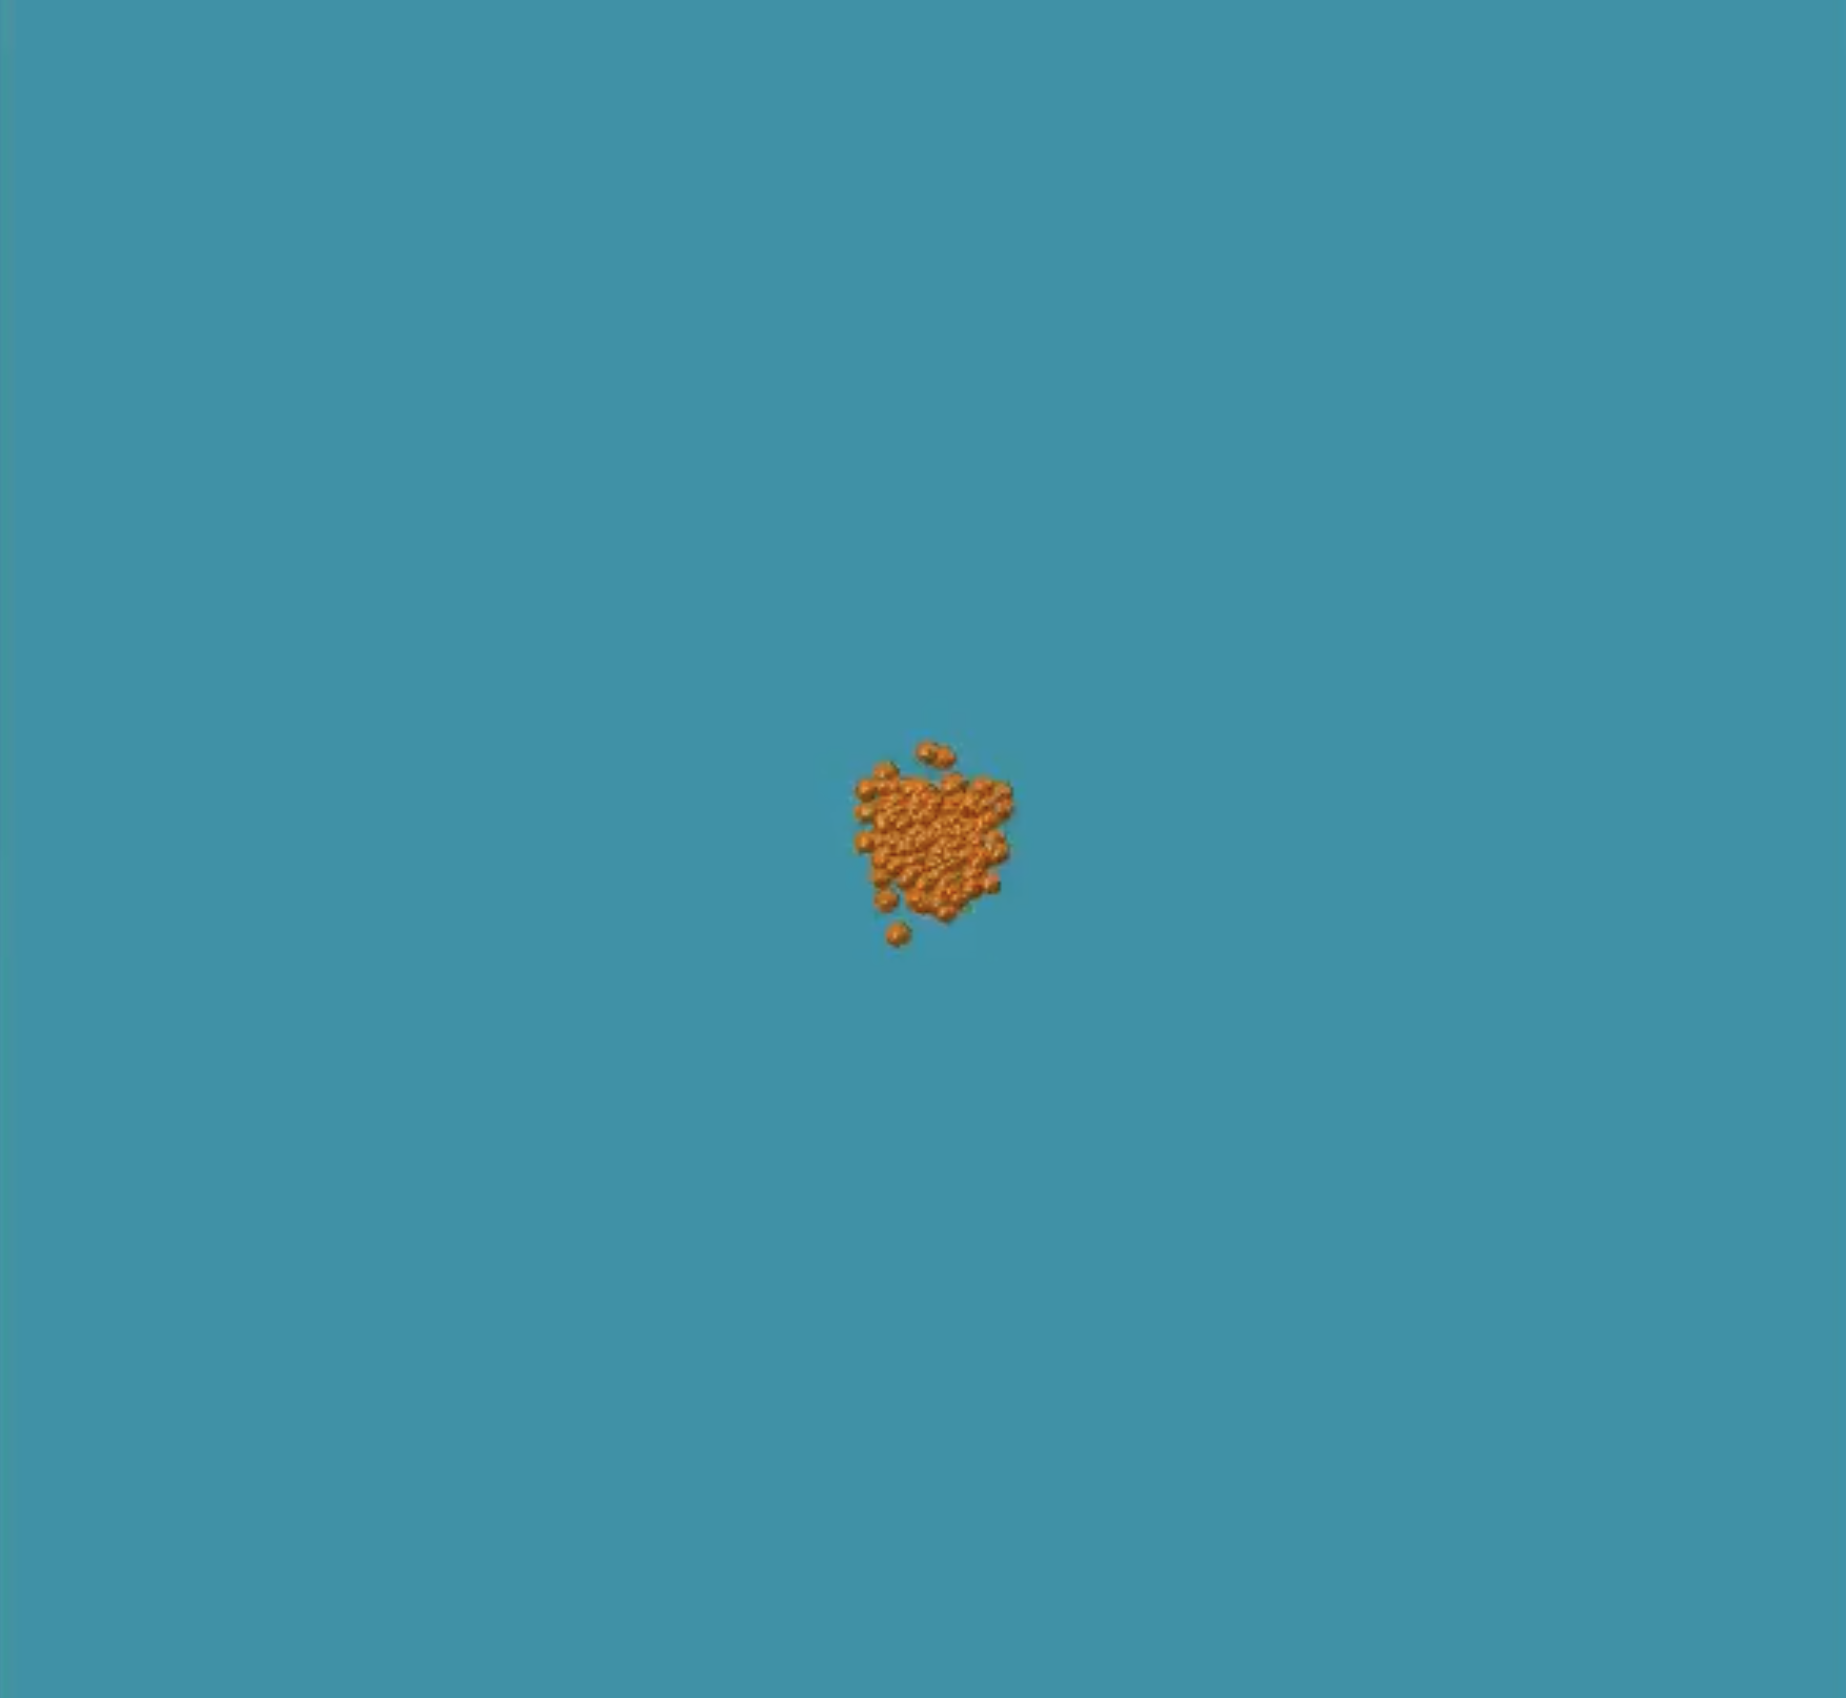
\includegraphics[width=0.25\textwidth]{../images/random_walk_particles_1} & 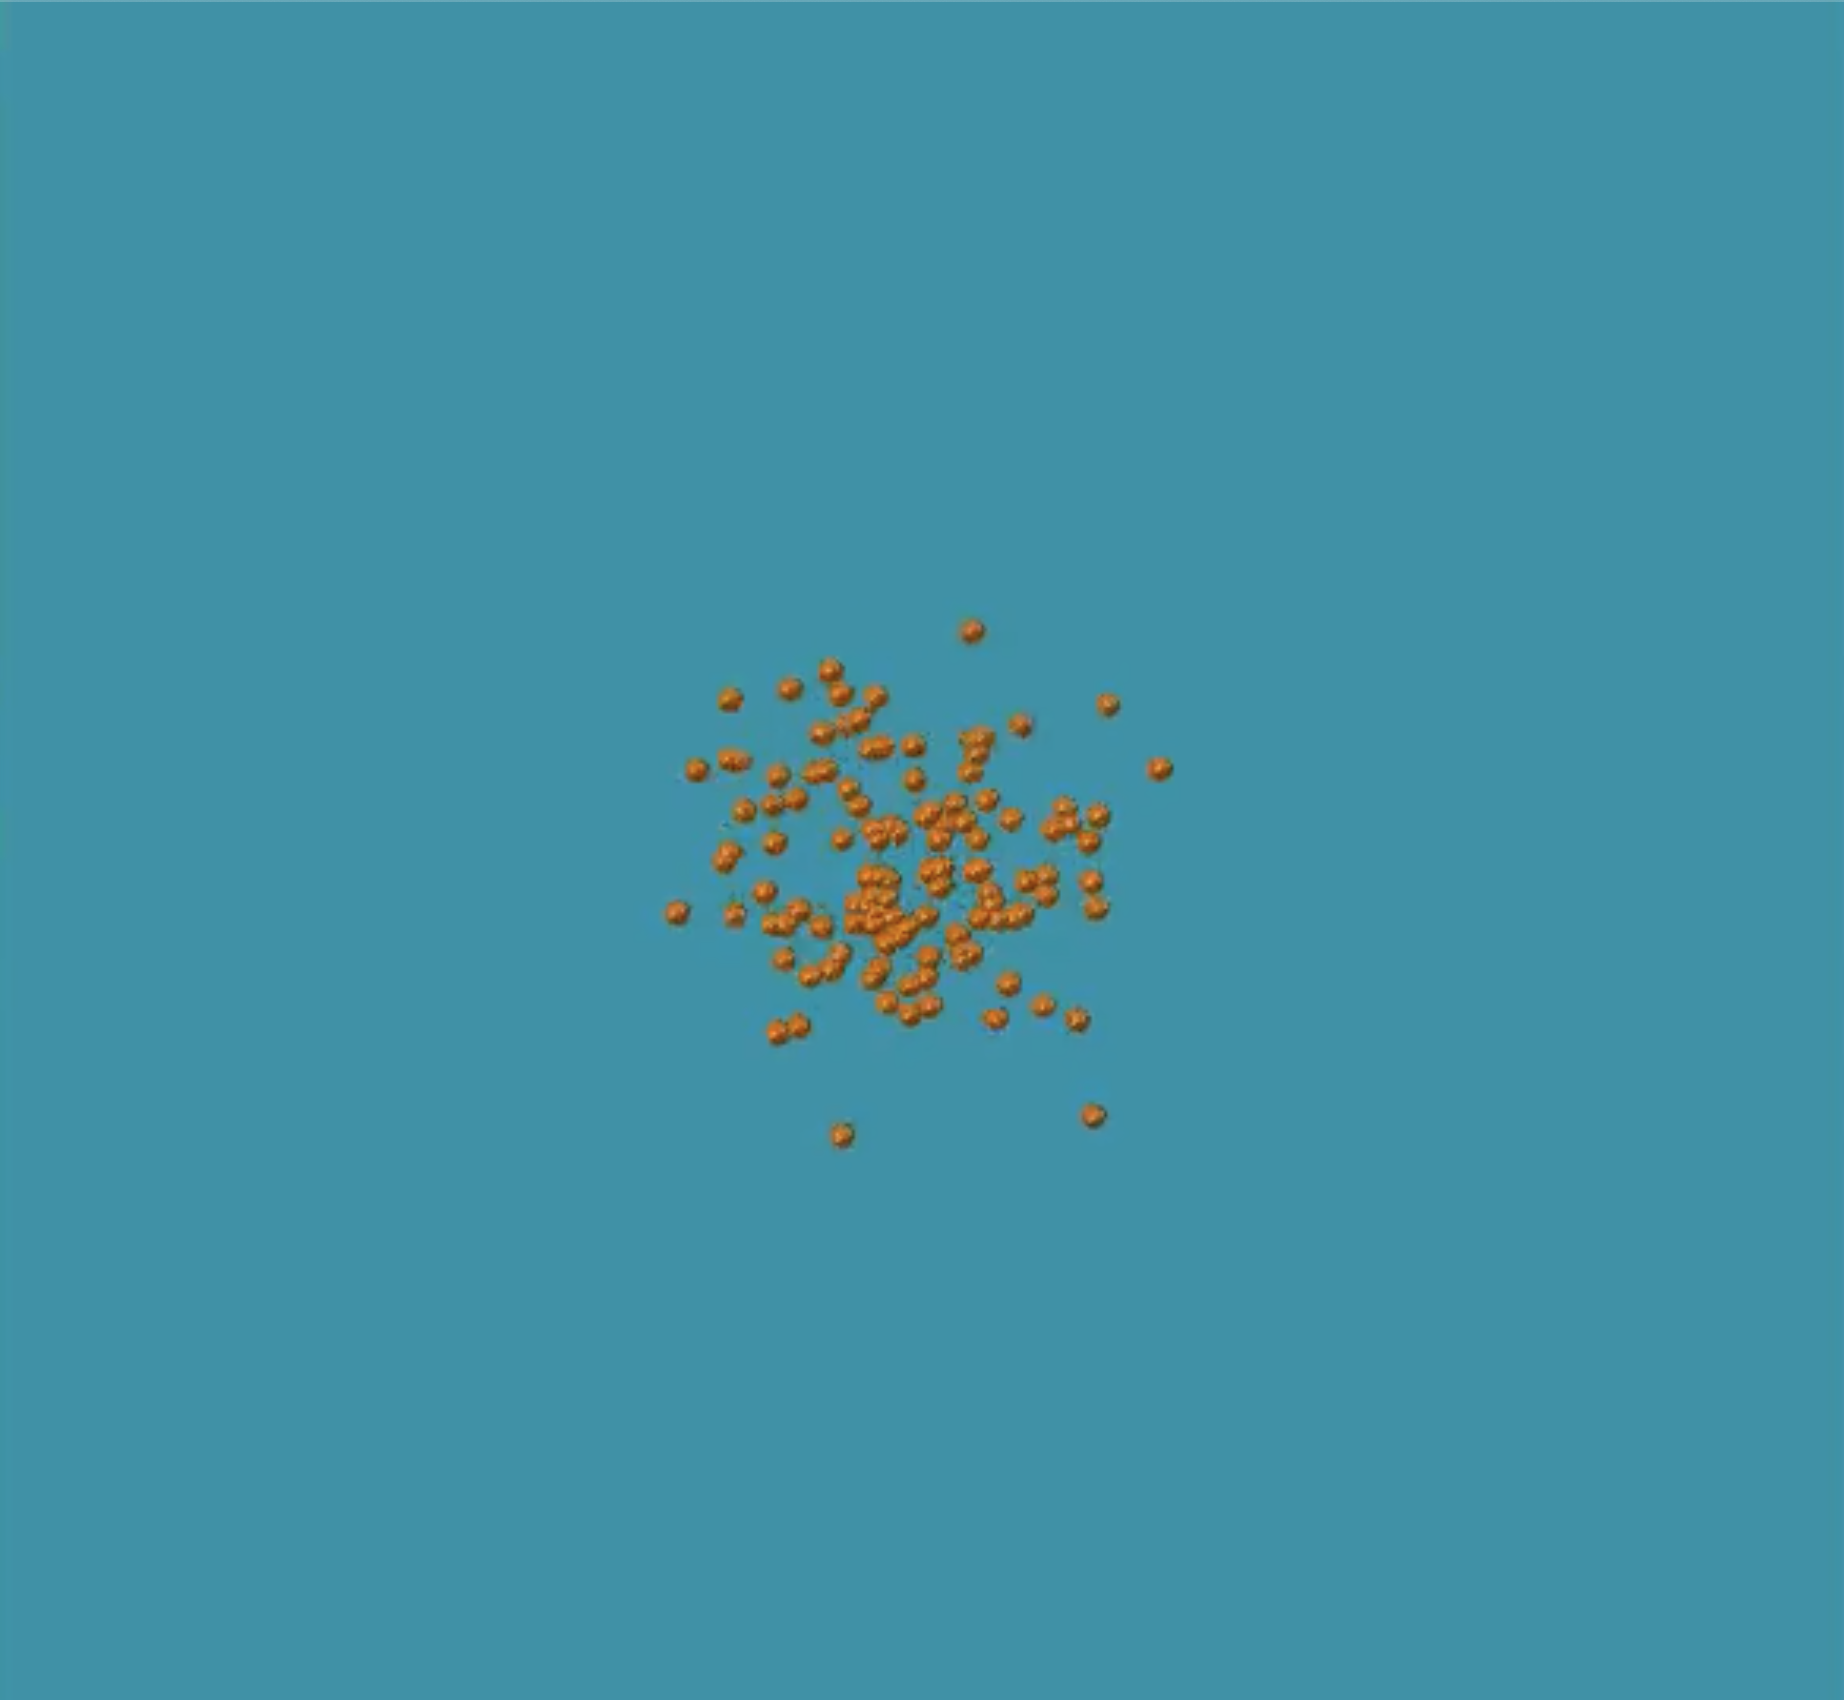
\includegraphics[width=0.25\textwidth]{../images/random_walk_particles_2} & 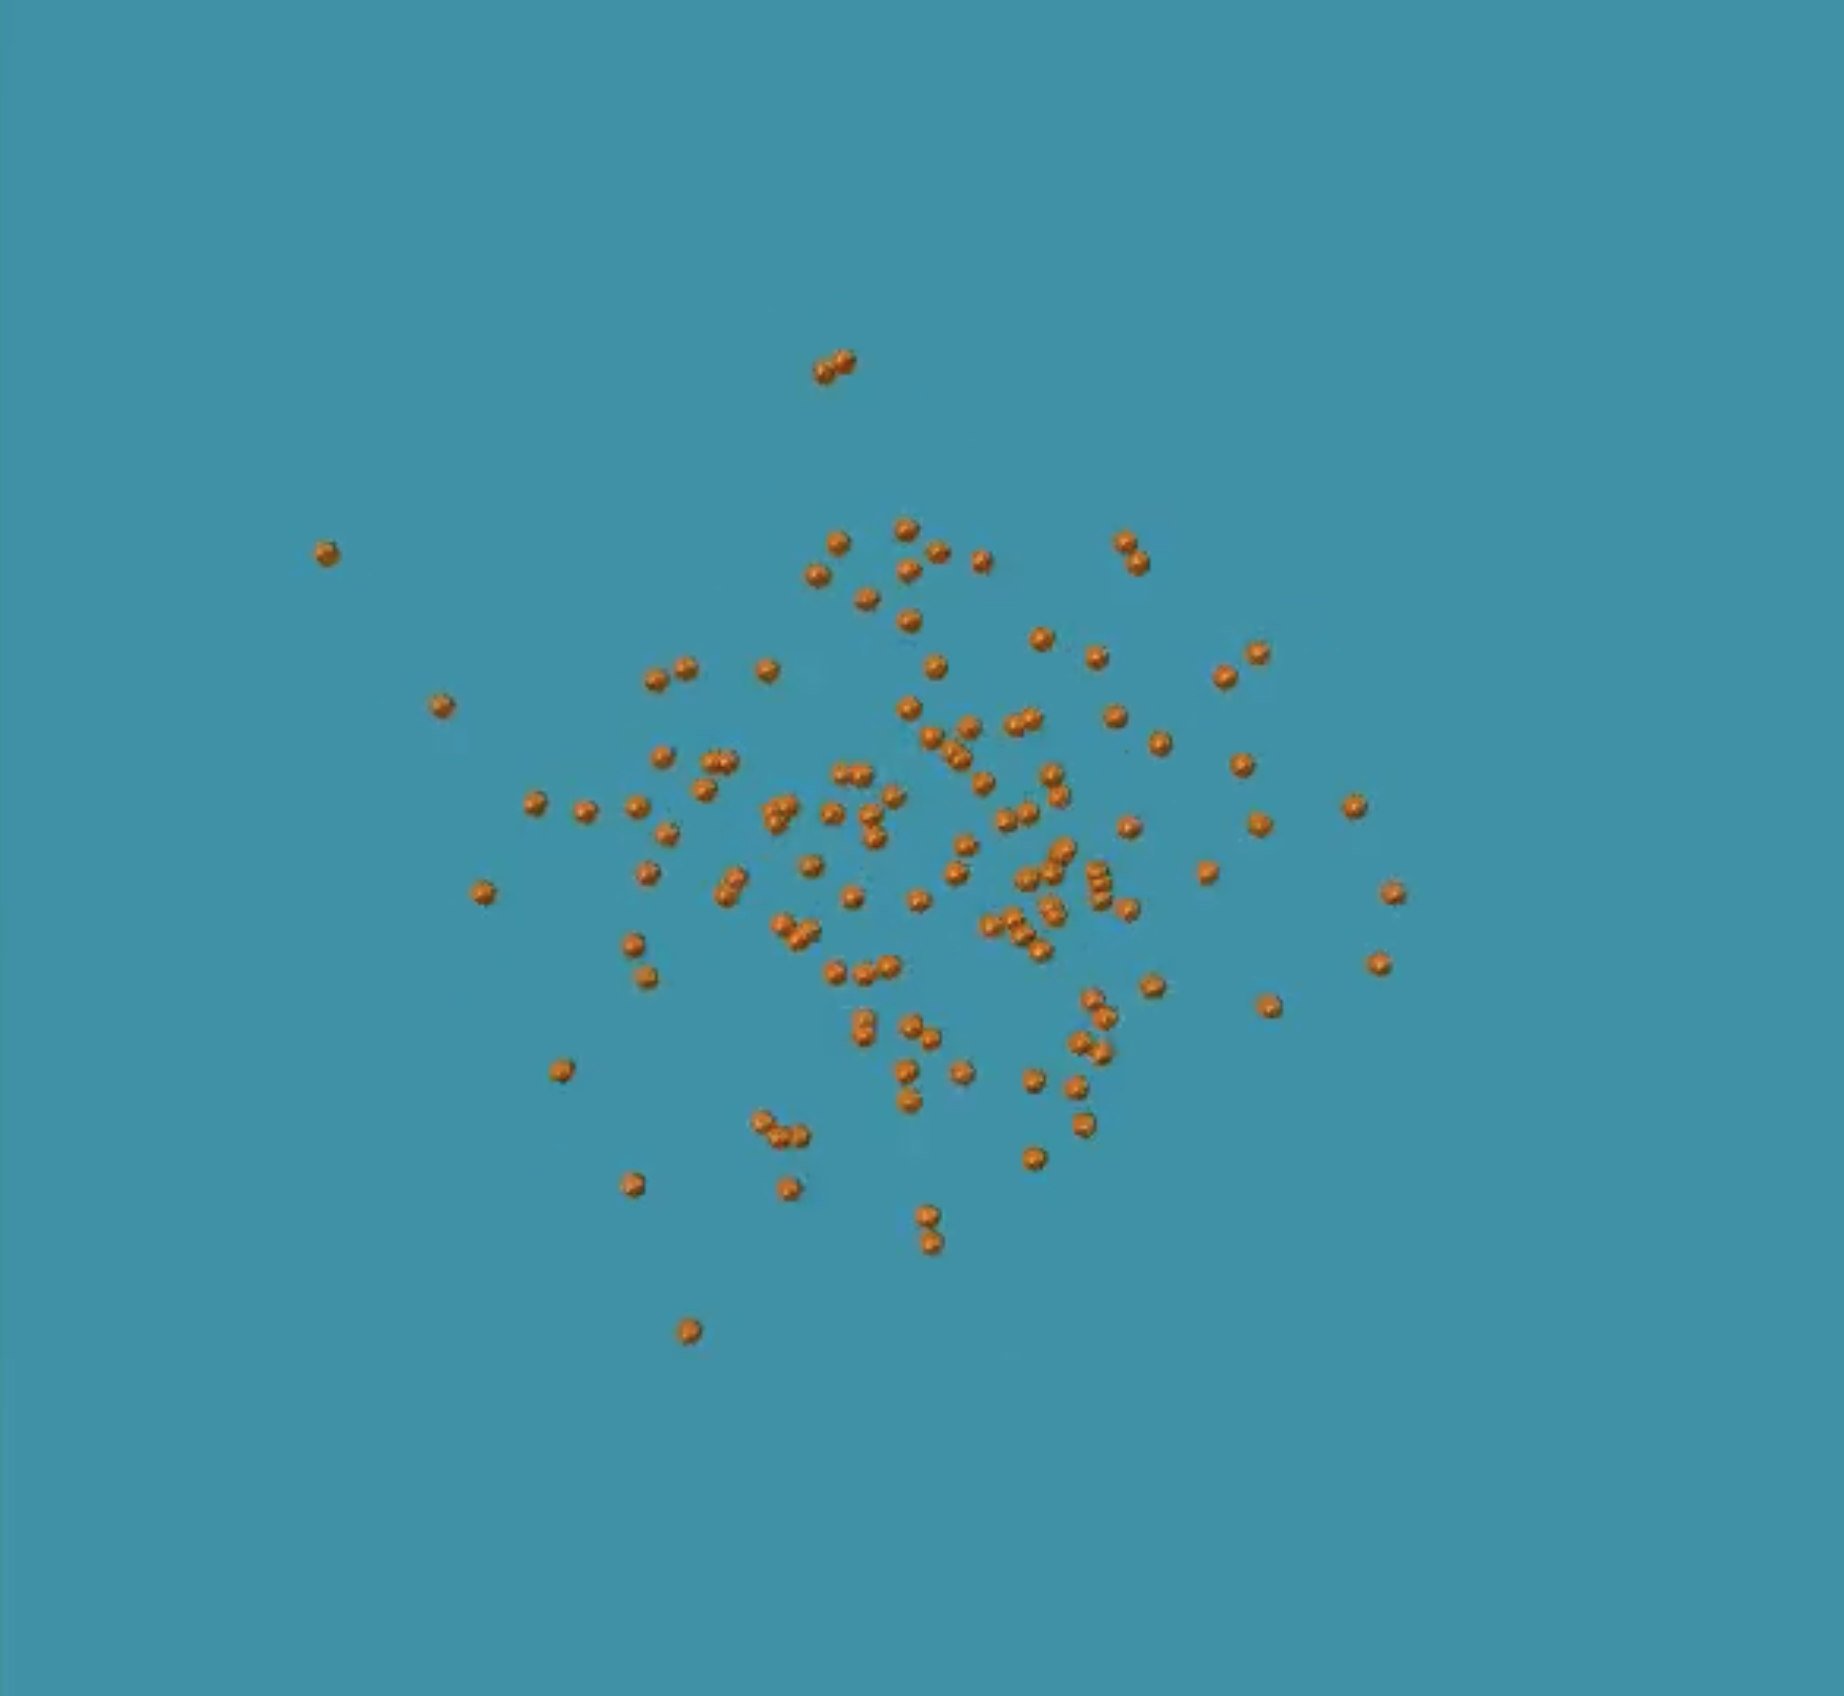
\includegraphics[width=0.25\textwidth]{../images/random_walk_particles_4}\\
\end{tabular}
\caption{Three time points captured from an animation of randomly walking particles all starting at the origin. As time advances from left to right, the points tend to drift outward.}
\label{fig:random_walk_multiple_particles}
\end{figure}

Although the movements of a single particle are random, we can draw conclusions about the \textit{average case} behavior of many particles can be predicted, as the following theorem indicates.

\begin{namedtheorem}[Random Walk]
After \textvar{n} steps of unit length in a random walk, a particle will on average find itself a distance from its origin that is proportional to $\sqrt{n}$.
\end{namedtheorem}

\fudgespace

\begin{note}[%
For readers who love mathematics, we provide a proof of the Random Walk Theorem in an appendix.
]\end{note}

Our experience of the world confirms the Random Walk Theorem's statement that randomly walking particles tend to drift away from their starting point. We understand, for example, that someone who has a respiratory virus can infect many others in an enclosed space in a short time frame. To take a less morbid example, we also know that when a cake is baking in the oven, we will not need to wait long for delicious smells to waft outward from the kitchen. But what does all this have to do with Alan Turing and zebra stripes?\\

\FloatBarrier
\phantomsection

\section{A Reaction-Diffusion Model Generating Turing Patterns}
\label{sec:a_reaction-diffusion_model_generating_turing_patterns}
\phantomsection

\subsection{From random walks to a reaction-diffusion system}

Turing's insight was that remarkable high-level patterns could arise if we combine particle diffusion with chemical reactions, in which colliding particles interact with each other. Such a model is called a \textdef{reaction-diffusion system}{reaction-diffusion system}{a model incorporating the diffusion of particles with chemical reactions involving these particles}, and the emergent patterns are called \textdef{Turing patterns}{Turing patterns}{patterns, such as stripes and spots, that emerge from certain reaction-diffusion systems} in Turing's honor.

We will consider a reaction-diffusion system having two types of particles, \textvar{A} and \textvar{B}. The system is not explicitly a predator-prey relationship, but you may like to think of the \textvar{A} particles as prey and the \textvar{B} particles as predators for reasons that will become clear soon.

Both types of particles diffuse randomly through the plane, but the \textvar{A} particles diffuse more quickly than the \textvar{B} particles.  In the simulation that follows, we will assume that \textvar{A} particles diffuse twice as quickly as \textvar{B} particles. In terms of our random walk model, this faster rate of diffusion means that in a single ``step'', an \textvar{A} particle moves twice as far as a \textvar{B} particle.\\

\begin{qbox}[%
Say that we release a collection of \textvar{A} and \textvar{B} particles at the same location. If the particles move via random walks, and the \textvar{A} particles diffuse twice as fast as the \textvar{B} particles, then on average, how much farther from the origin will the \textvar{A} particles be than the \textvar{B} particles after \textvar{n} steps?
]\end{qbox}

We now will add three reactions to our system, which are illustrated in \autoref{fig:three_reactions}. First, \textvar{A} particles are added into the system at some constant \textdefnogloss{feed rate} \textvar{f}. As a result of the feed reaction, the concentration of the \textvar{A} particles increases by a constant in each time step.\\

\begin{note}[%
We will work with a two-dimensional simulation, but in a three-dimensional system, the units of \textvar{f} would be in mol/L/s, which means that every second, there are \textvar{f} moles of particles added to the system for every liter of volume. (Recall from your chemistry class long ago that one mole is $6.02214076 \cdot 10^{23}$ particles, called Avogadro's number.)
]\end{note}

Second, \textvar{B} particles are removed from the system at a constant \textdefnogloss{kill rate} \textvar{k}. As a result of the kill reaction, the number of \textvar{B} particles in the system will decrease by a factor of \textvar{k} in a given time step. That is, the more \textvar{B} particles that are present, the more \textvar{B} particles will be removed.

Third, our reaction-diffusion system includes the following reaction involving both particle types. The particles on the left side of this reaction are called \textdef{reactants}{reactants}{substances taking part in a reaction} and the particles on the right side are called \textdef{products}{products}{substances resulting from a reaction}.

\begin{center}
$A + 2B \rightarrow 3B$
\end{center}

To simulate this reaction on a particle level, if an \textvar{A} particle and two \textvar{B} particles collide with each other, then the \textvar{A} particle has some fixed probability of being replaced by a third \textvar{B} particle, which could vary based on the presence of a catalyst and the orientation of the particles. This probability directly relates to the \textit{rate} at which this reaction occurs. This third reaction is why we compared \textvar{A} to prey and \textvar{B} to predators, since we may like to conceptualize the reaction as two \textvar{B} particles consuming an \textvar{A} particle and producing an offspring \textvar{B} particle.\\

\begin{figure}[h]
\centering
\mySfFamily
\tabcolsep=2em
\begin{tabular}{c c}
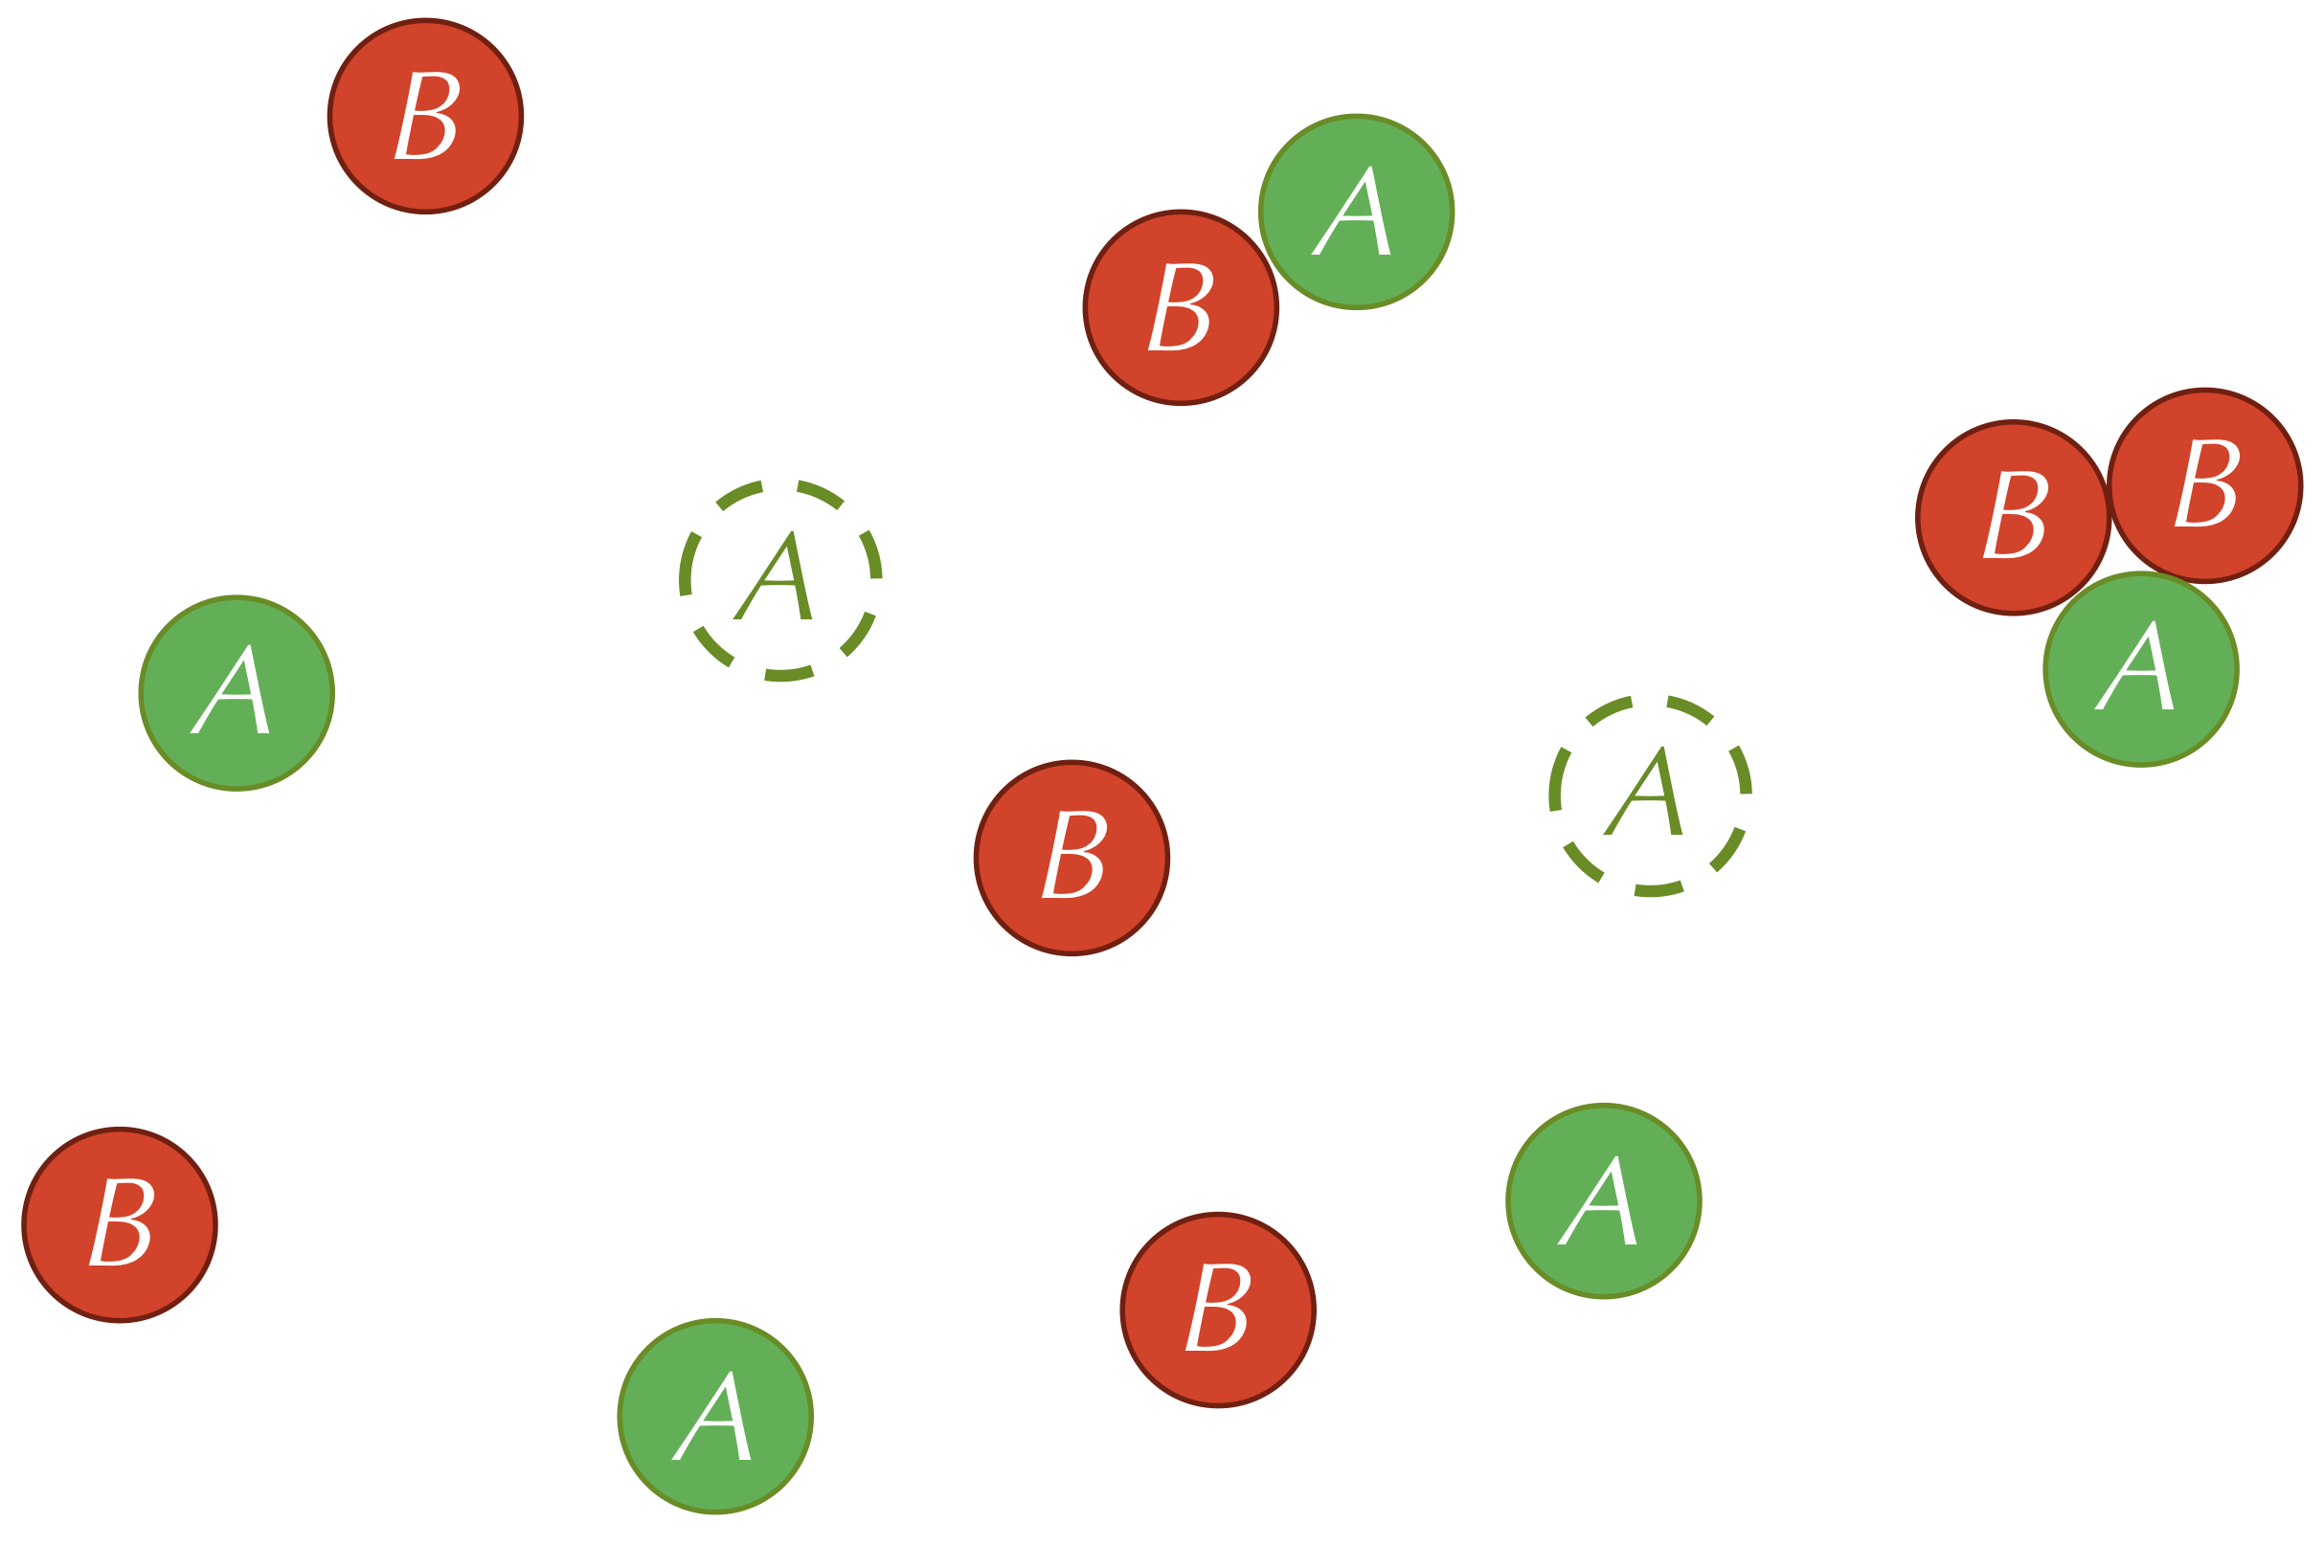
\includegraphics[width=0.35\textwidth]{../images/reaction-diffusion_three_reactions_before} & 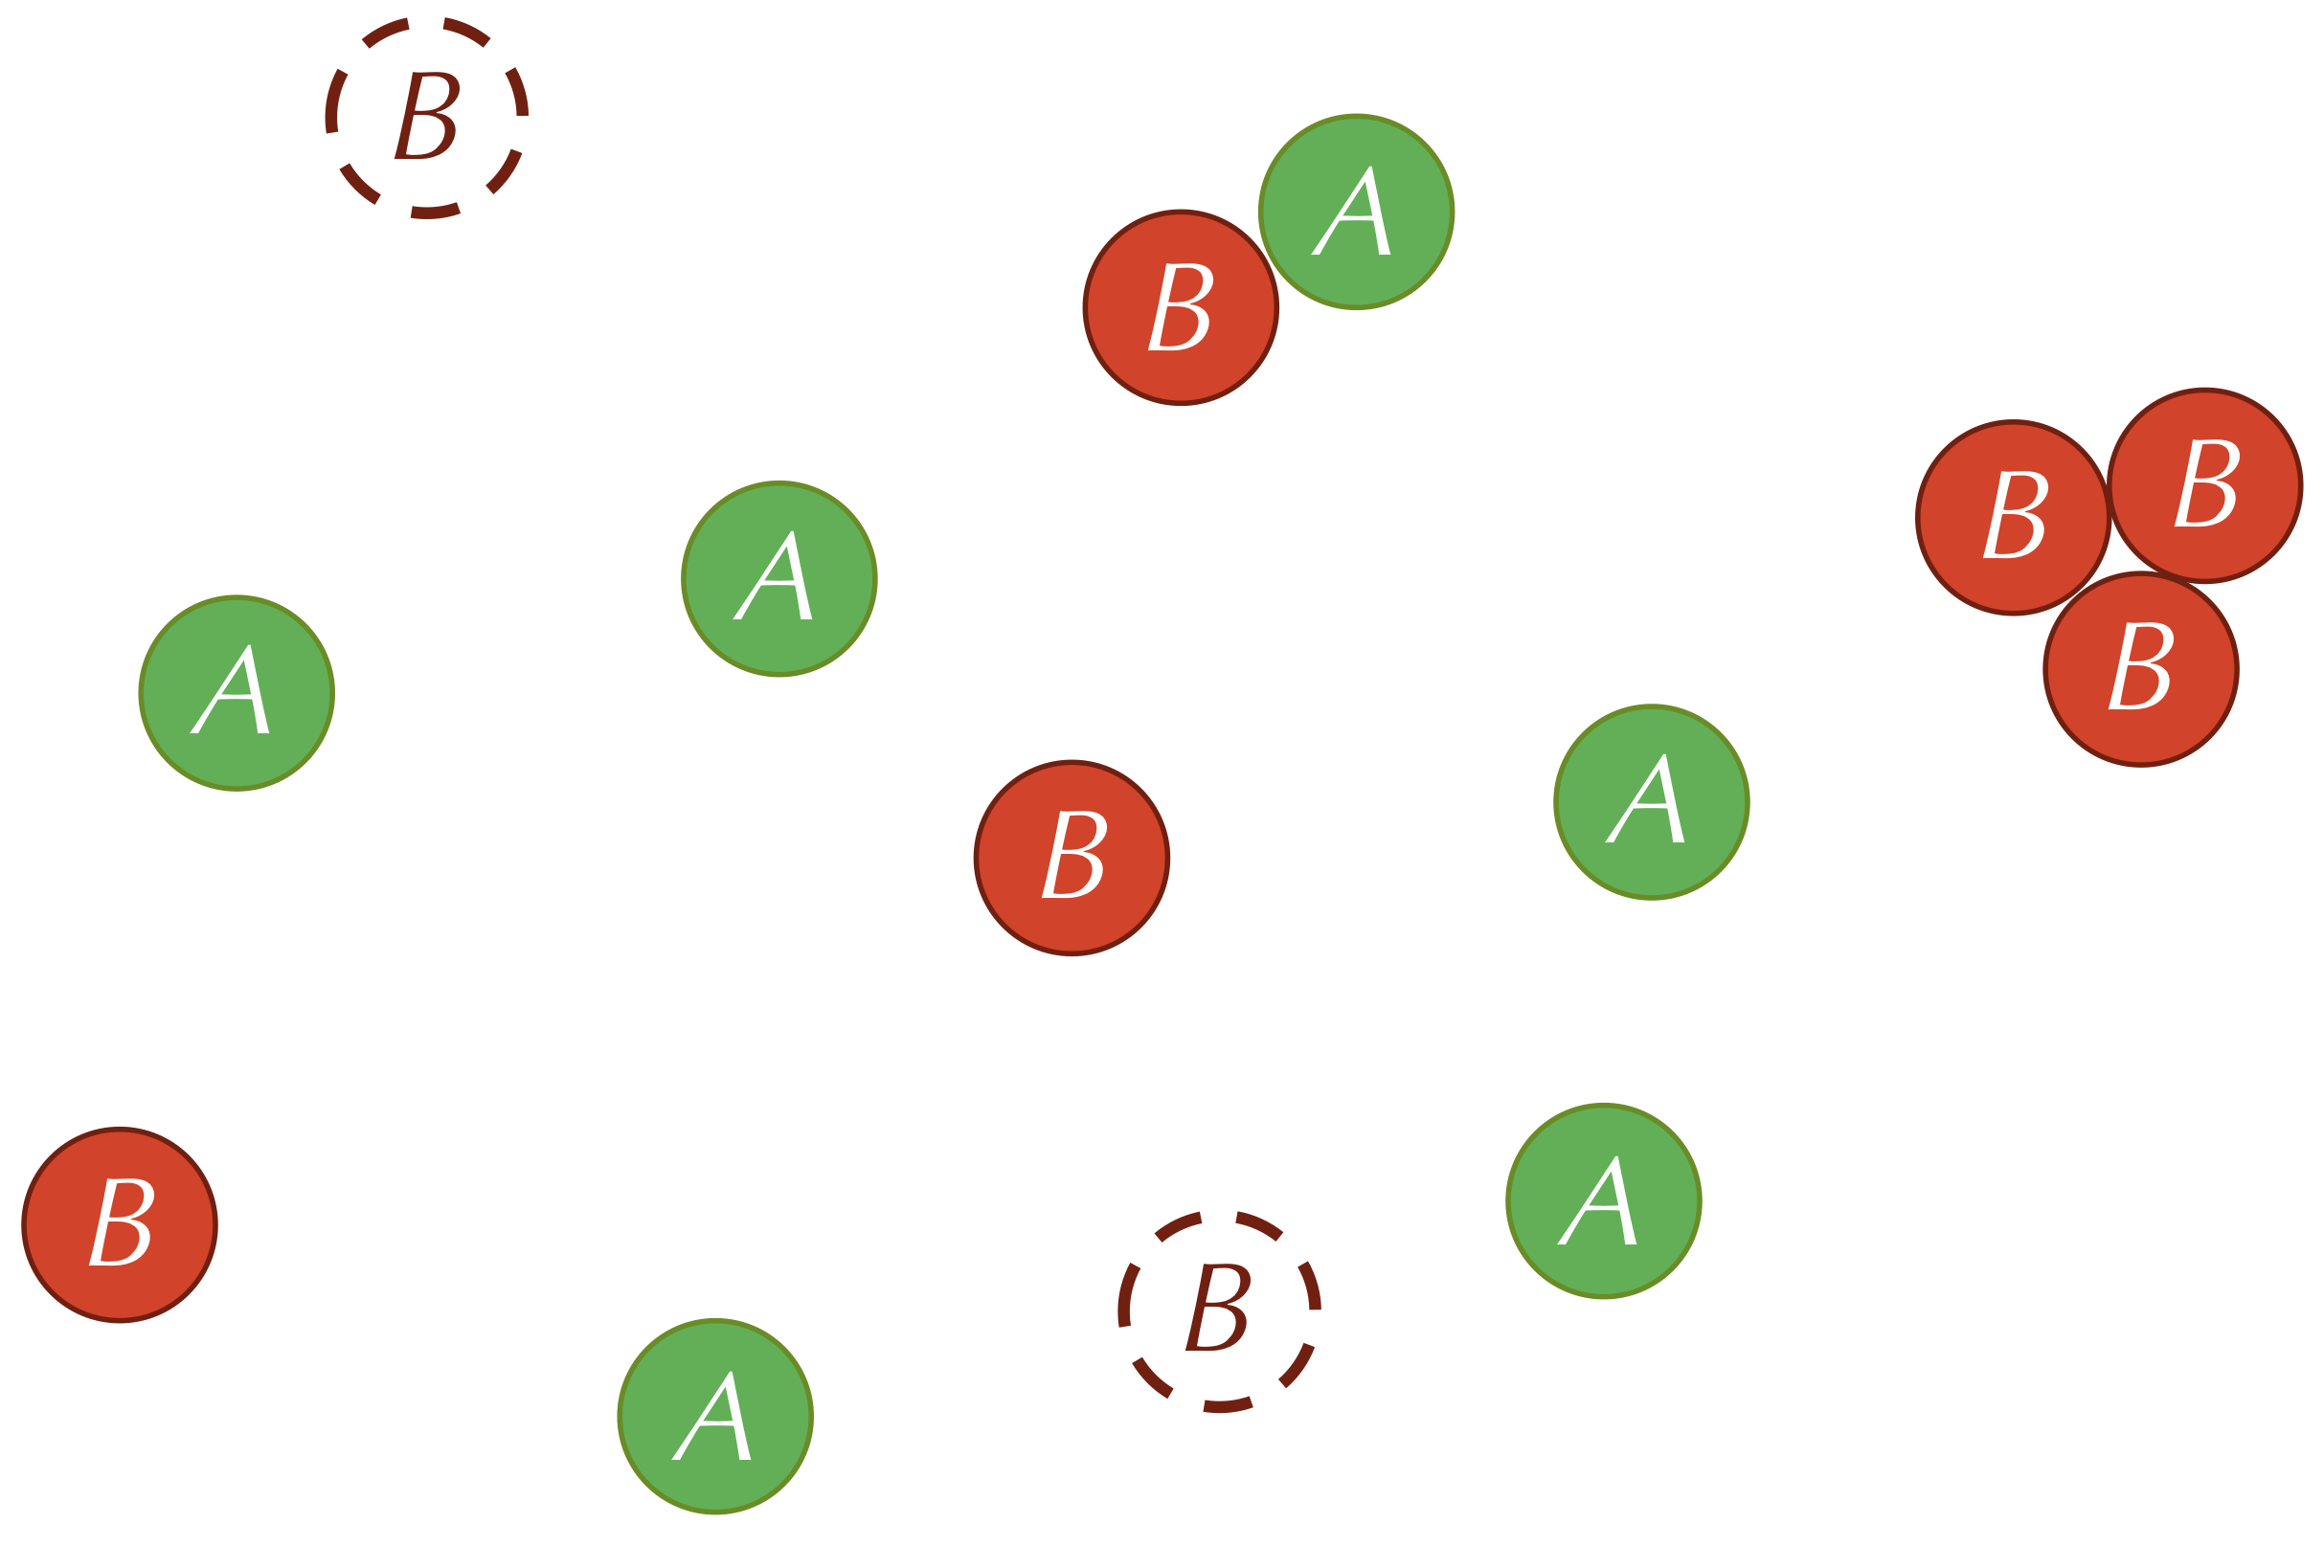
\includegraphics[width=0.35\textwidth]{../images/reaction-diffusion_three_reactions_after}\\
\end{tabular}
\caption{A visualization of our reaction-diffusion system. (Left) The system contains both types of particles and two collisions of particles. The two \textvar{A} particles shown with dashed lines are not yet present.  (Right) Two \textvar{A} particles are fed into the system, two of the \textvar{B} particles die out, and a \textvar{B} particle replaces an \textvar{A} particle after the collision of two \textvar{B} particles and an \textvar{A} particle.}
\label{fig:three_reactions}
\end{figure}

Before continuing, we call your attention to a slight difference between the feed and kill reactions. In the former, the concentration of \textvar{A} particles increases by a constant in each time step. In the latter, the concentration of \textvar{B} particles decreases by a constant factor multiplied by the current concentration of \textvar{B} particles. If we were using calculus to model this system, then letting [\textvar{A}] and [\textvar{B}] denote the concentrations of the two particle types, we would represent the feed and kill reactions by the following two differential equations:
\begin{align*}
\dfrac{\mathrm{d}[A]}{\mathrm{d}t} & = f\\[1ex]
\dfrac{\mathrm{d}[B]}{\mathrm{d}t} & = k \cdot [B]\,.
\end{align*}

\FloatBarrier
\phantomsection
\subsection{Parameters are omnipresent in biological modeling}

A \textdef{parameter}{parameter}{a variable used as input to a model} is a variable quantity used as input to a model. Parameters are inevitable in biological modeling (and data science in general), and as we will see, changing parameters can cause major changes in the behavior of a system.

Four parameters are relevant to our reaction-diffusion system: the feed rate (\textvar{f}) of \textvar{A} particles, the kill rate (\textvar{k}) of the \textvar{B} particles, the predator-prey reaction rate (\textvar{r}), and the diffusion rate (i.e., speed) of the the \textvar{B} particles. We do not need to set the diffusion rate of the \textvar{A} particles, since we know that their diffusion is twice that of the \textvar{B} particles.

\begin{qbox}[%
What will happen as we increase or decrease \textvar{f} or \textvar{k}?
]\end{qbox}

We think of all these parameters as dials that we can turn, observing how the system changes as a result. For example, if we raise the diffusion rate, then the particles will be moving around and colliding with each other more, which means that we will see more of the reaction $\textvar{A} + 2\textvar{B} \rightarrow 3\textvar{B}$. We will then initiate our reaction-diffusion system with a uniform concentration of \textvar{A} particles spread across the grid and a tightly packed collection of \textvar{B} particles in the center of the grid. As the \textvar{B} particles diffuse, what will we see?\tutorial[prologue/turing-cellblender]\\

\FloatBarrier
\phantomsection
\subsection{Changing reaction-diffusion parameters yields different Turing patterns}



For many parameter values, our reaction-diffusion system is not very interesting. \autoref{fig:k=500000_f=1000} shows that if the kill rate is too high, then the \textvar{B} particles (colored red) will die out more quickly than they can be replenished by the reaction with \textvar{A} particles (colored green), and so only \textvar{A} particles will remain.

\begin{figure}[h]
\centering
\mySfFamily
\begin{tabular}{c c c c}
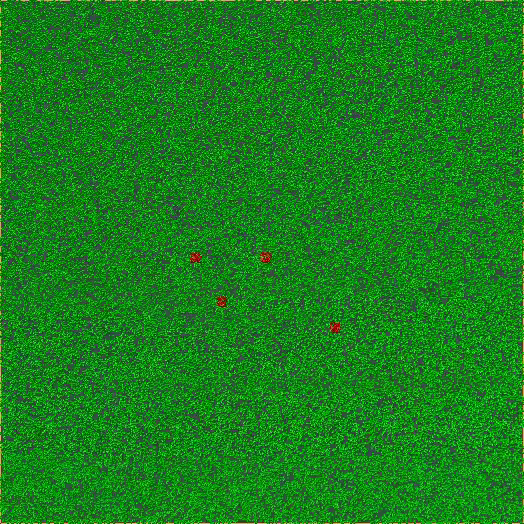
\includegraphics[width = 0.2\textwidth]{../images/predator_prey_predator_dies_f1e1_r5e5.png} & 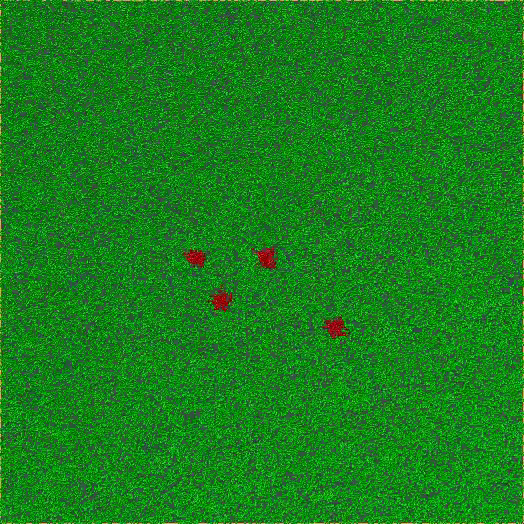
\includegraphics[width = 0.2\textwidth]{../images/../images/predator_prey_predator_dies_f1e1_r5e5_i1.png} & 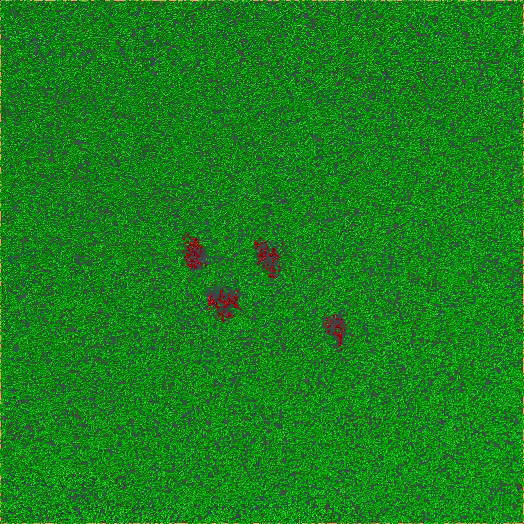
\includegraphics[width = 0.2\textwidth]{../images/../images/predator_prey_predator_dies_f1e1_r5e5_i2.png} & 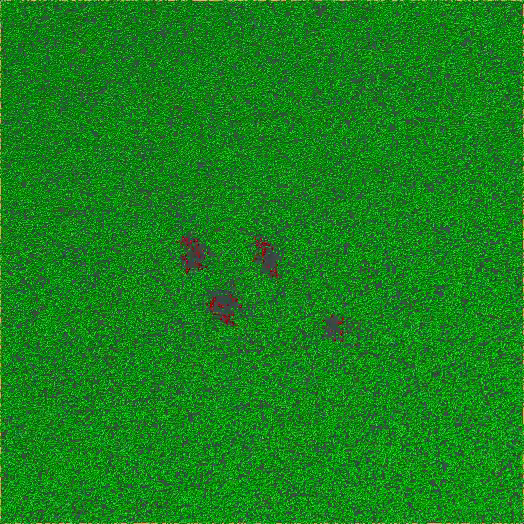
\includegraphics[width = 0.2\textwidth]{../images/../images/predator_prey_predator_dies_f1e1_r5e5_i3.png}\\[2ex]
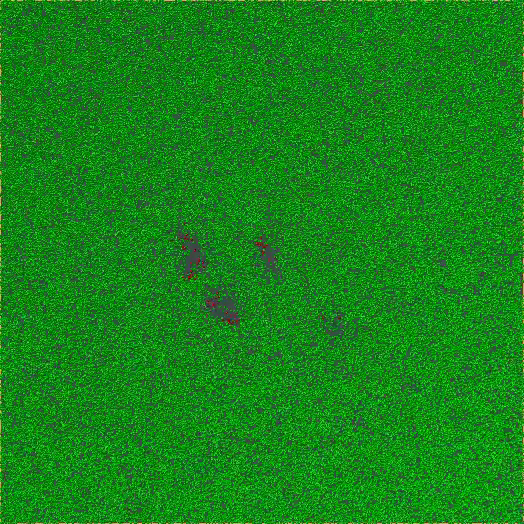
\includegraphics[width = 0.2\textwidth]{../images/predator_prey_predator_dies_f1e1_r5e5_i4.png} & 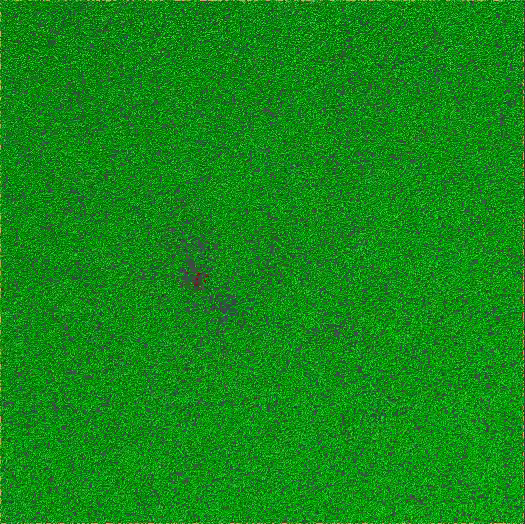
\includegraphics[width = 0.2\textwidth]{../images/../images/predator_prey_predator_dies_f1e1_r5e5_i5.png} & 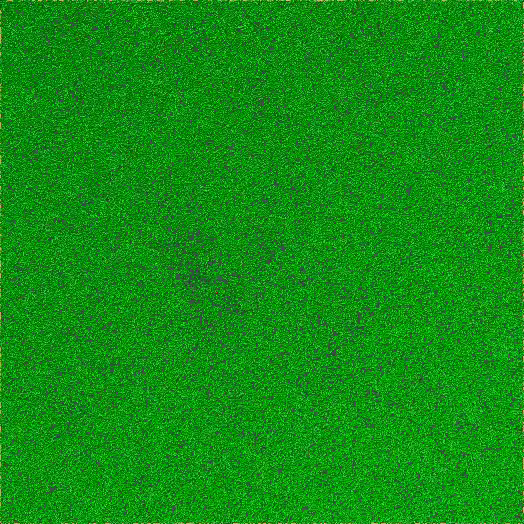
\includegraphics[width = 0.2\textwidth]{../images/../images/predator_prey_predator_dies_f1e1_r5e5_i6.png} & 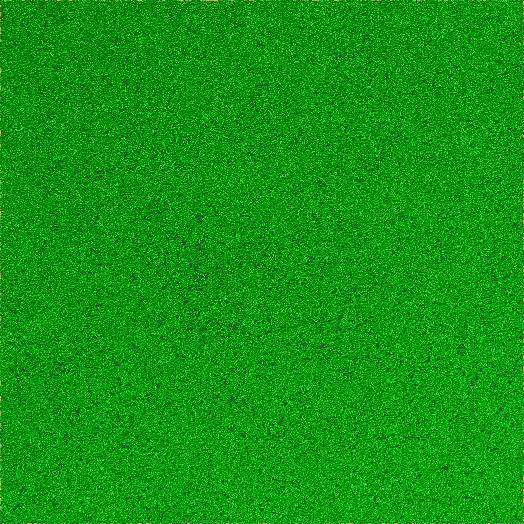
\includegraphics[width = 0.2\textwidth]{../images/../images/predator_prey_predator_dies_f1e1_r5e5_i7.png}
\end{tabular}
\caption{An eight-panel animation of a CellBlender simulation of our reaction-diffusion system using the parameter rates \textvar{f} = 1,000 and \textvar{k} = 500,000. As the animation proceeds (from top left to bottom right), small pockets of \textvar{B} particles form, but they die out more quickly than they can be replenished, leaving only \textvar{A} particles.}
\label{fig:k=500000_f=1000}
\end{figure}

On the other hand, \autoref{fig:k=100000_f=1000000} shows that if \textvar{f} is too high, then the increased feed rate will cause an increase in the concentration of \textvar{A} particles. However, the increased concentration of \textvar{A} particles will also cause more interactions between \textvar{A} particles and pairs of \textvar{B} particles, causing the concentration of \textvar{B} particles to explode.

\begin{figure}[h]
\centering
\mySfFamily
\begin{tabular}{c c c c}
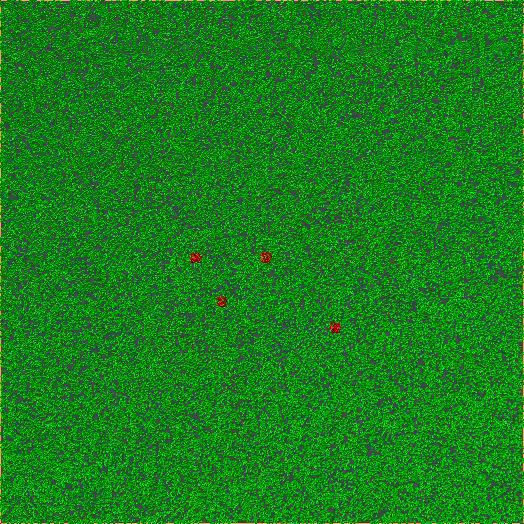
\includegraphics[width = 0.2\textwidth]{../images/predator_prey_f1e6_d1e5.png} & 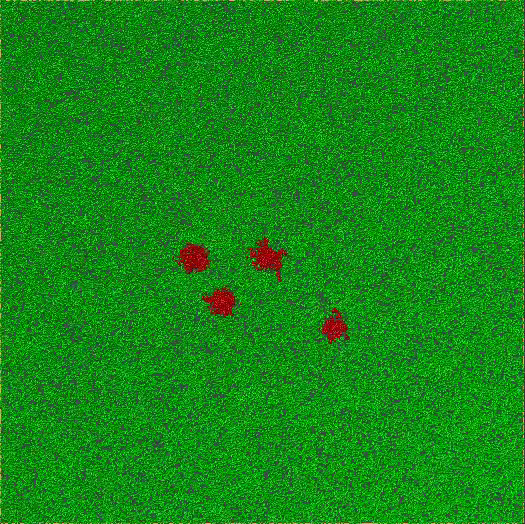
\includegraphics[width = 0.2\textwidth]{../images/../images/predator_prey_f1e6_d1e5_i1.png} & 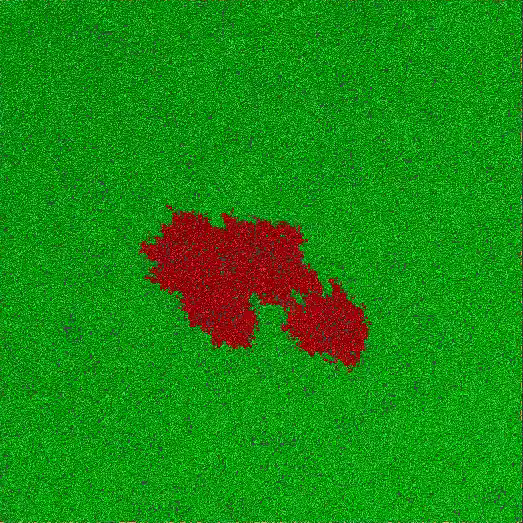
\includegraphics[width = 0.2\textwidth]{../images/../images/predator_prey_f1e6_d1e5_i2.png} & 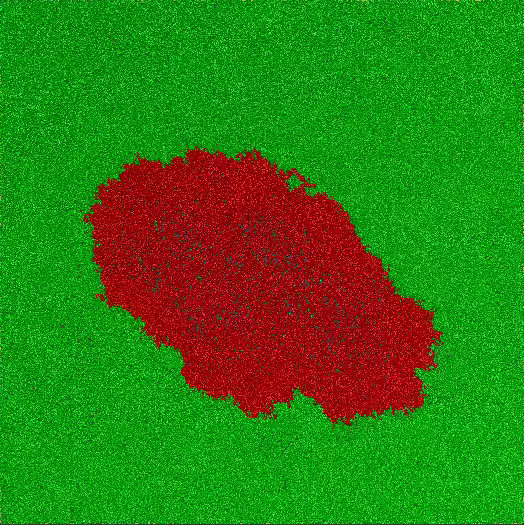
\includegraphics[width = 0.2\textwidth]{../images/../images/predator_prey_f1e6_d1e5_i3.png}\\[2ex]
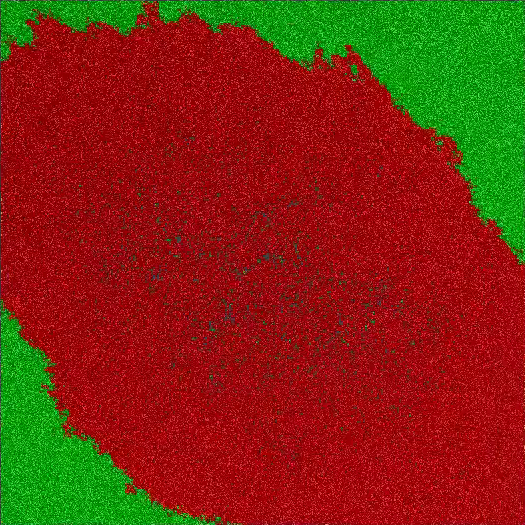
\includegraphics[width = 0.2\textwidth]{../images/predator_prey_f1e6_d1e5_i4.png} & 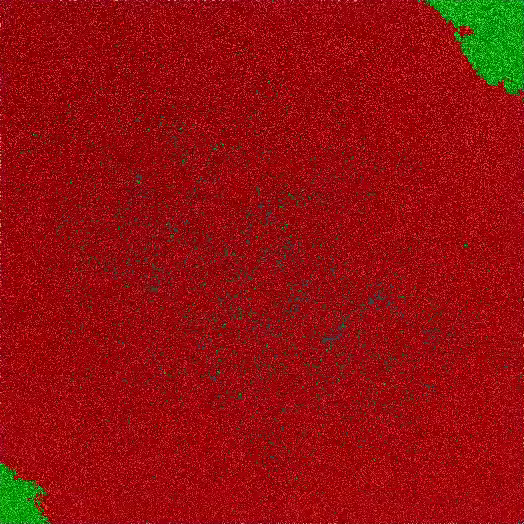
\includegraphics[width = 0.2\textwidth]{../images/../images/predator_prey_f1e6_d1e5_i5.png} & 
\includegraphics[width = 0.2\textwidth]{../images/../images/predator_prey_f1e6_d1e5_i6.png} & 
\includegraphics[width = 0.2\textwidth]{../images/../images/predator_prey_f1e6_d1e5_i7.png}
\end{tabular}
\caption{An animation of a CellBlender simulation of our reaction-diffusion system using the parameter rates \textvar{f} = 1,000,000 and \textvar{k} = 100,000. Because of the high feed rate and low kill rate, the ``predator'' \textvar{B} particles expand rapidly and achieve higher concentration than the \textvar{A} particles across the system.}
\label{fig:k=100000_f=1000000}
\end{figure}

The interesting behavior in this system lies in a sweet spot in which the \textvar{f} and \textvar{k} parameters are closer to each other. With such a simulation, \autoref{fig:k=200000_f=100000} shows a clear stripe of predators expanding outward against a background of prey, with subsequent stripes appearing at locations where a critical mass of predators can interact with each other.

\begin{figure}[h]
\centering
\mySfFamily
\begin{tabular}{c c c c}

\includegraphics[width = 0.2\textwidth]{../images/predator_prey_11_by_11_f_1_k_2.png} & 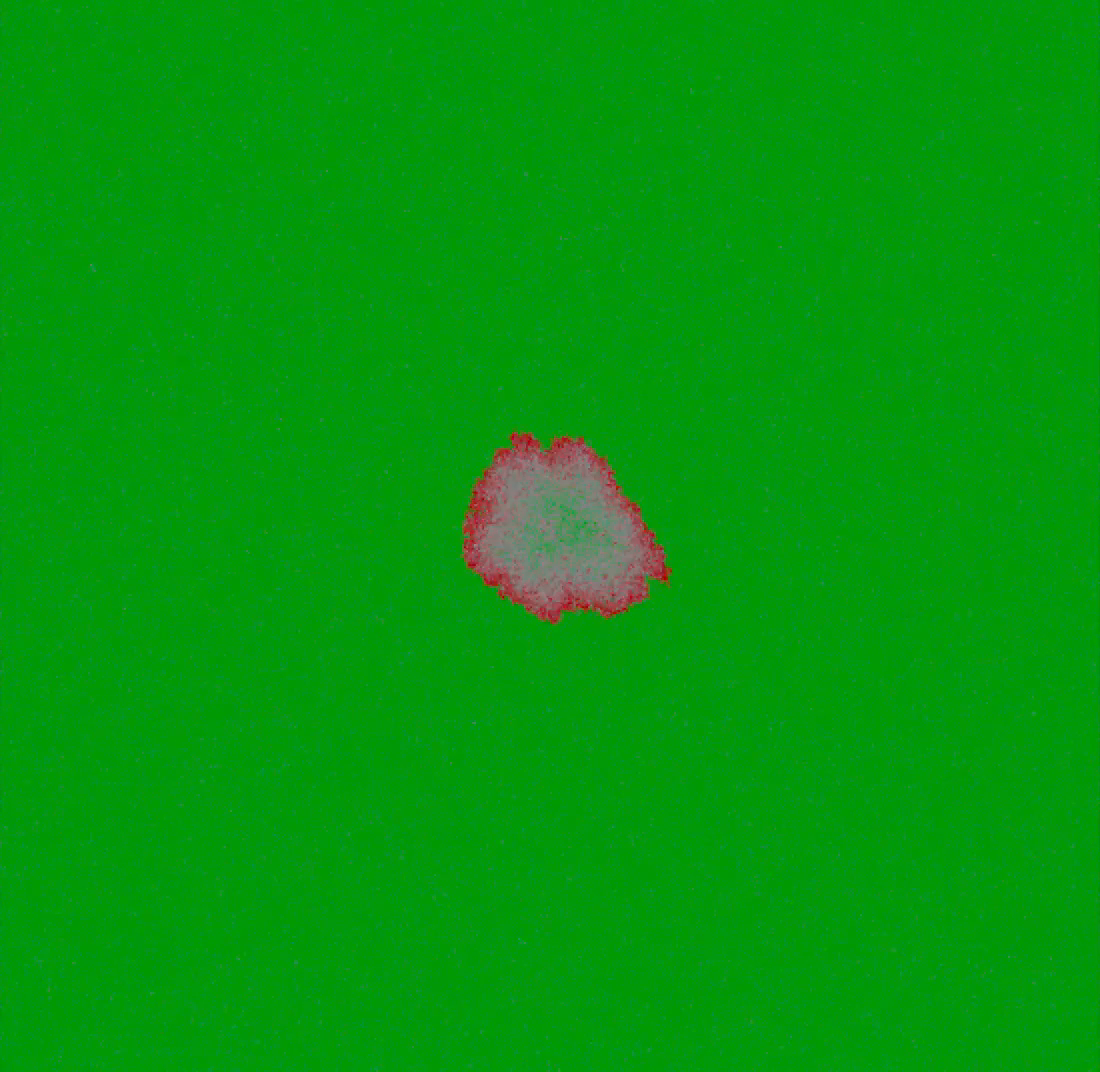
\includegraphics[width = 0.2\textwidth]{../images/../images/predator_prey_11_by_11_f_1_k_2_i1.png} & 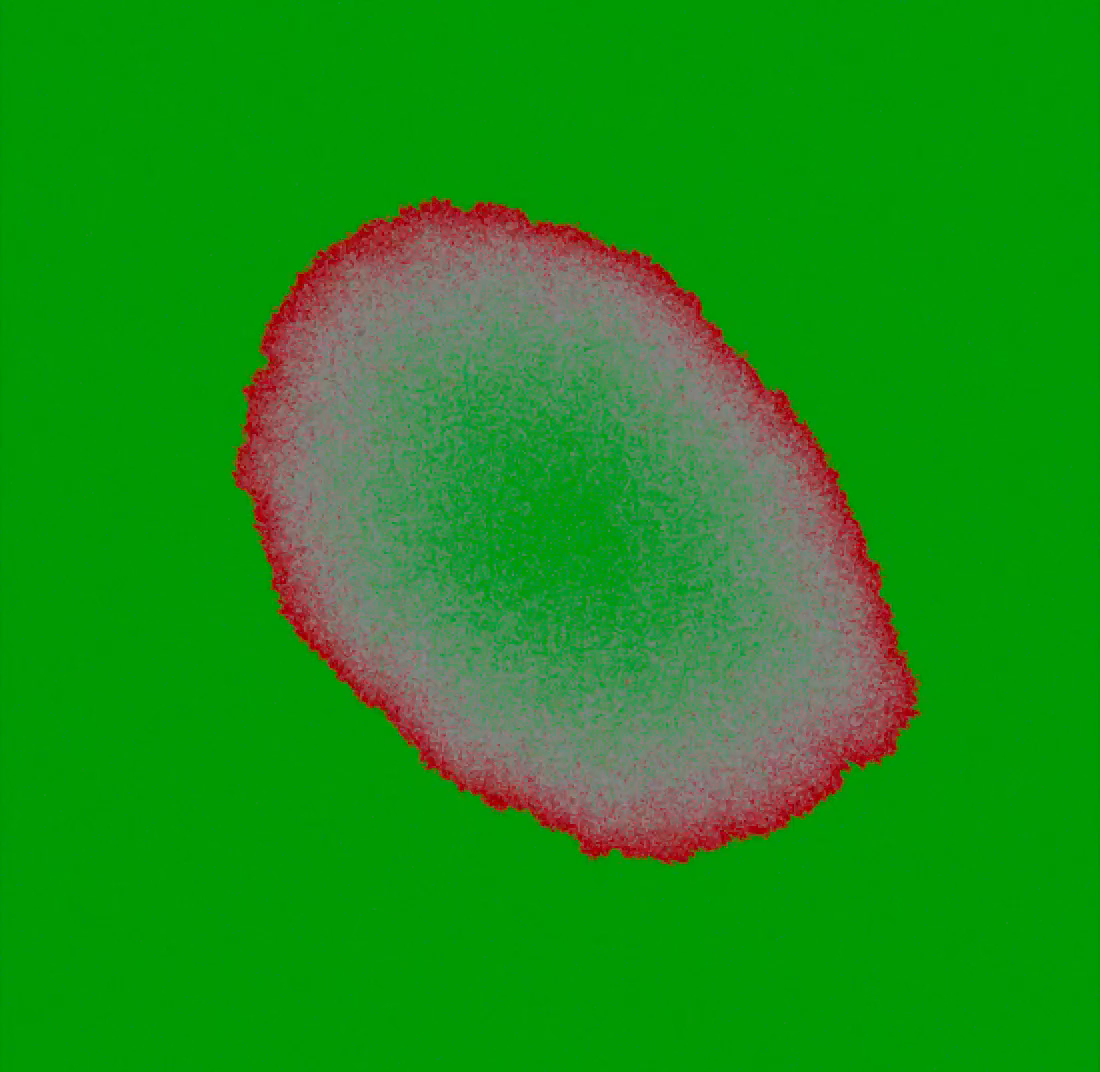
\includegraphics[width = 0.2\textwidth]{../images/../images/predator_prey_11_by_11_f_1_k_2_i2.png} & 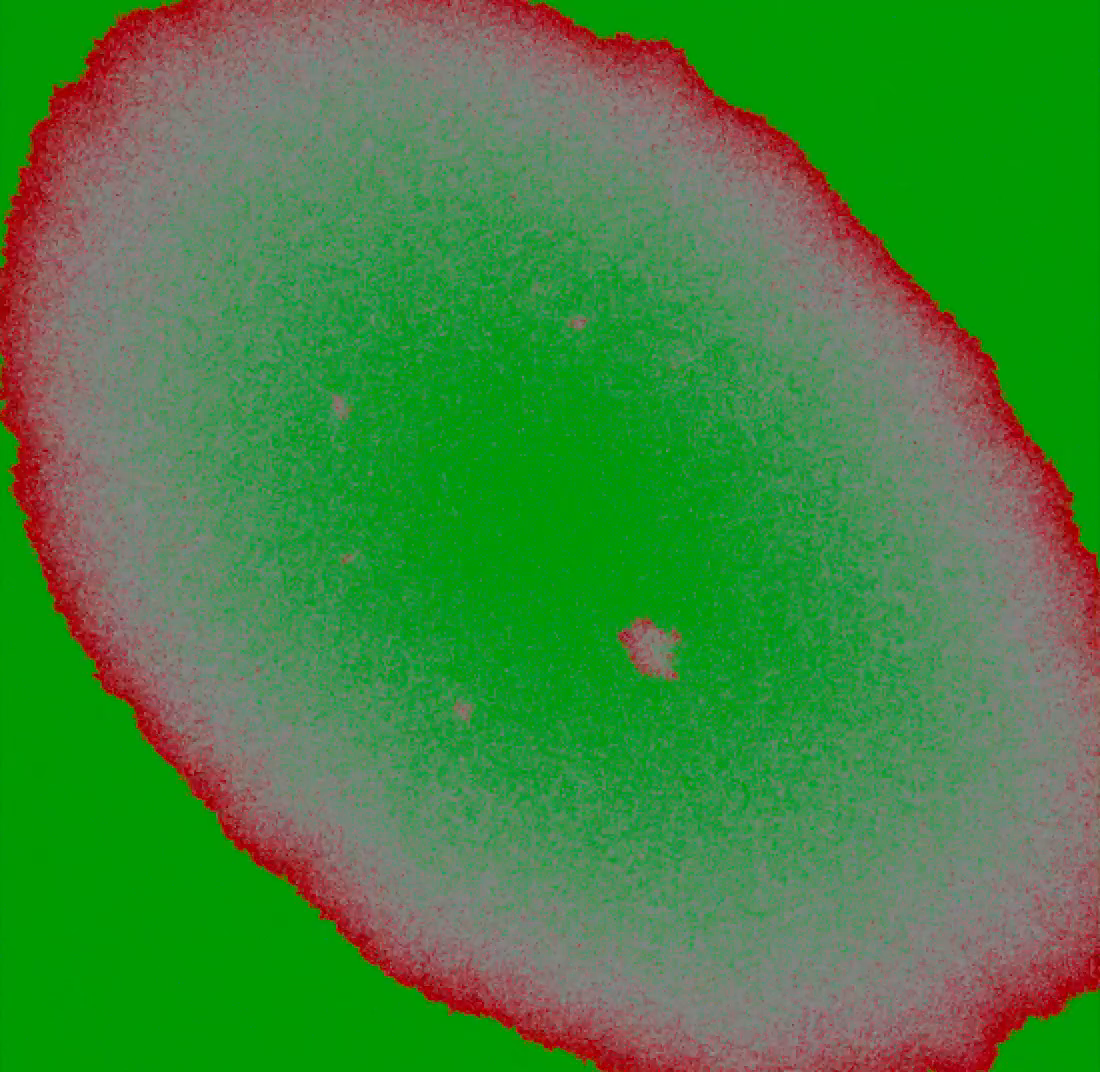
\includegraphics[width = 0.2\textwidth]{../images/../images/predator_prey_11_by_11_f_1_k_2_i3.png}\\[2ex]
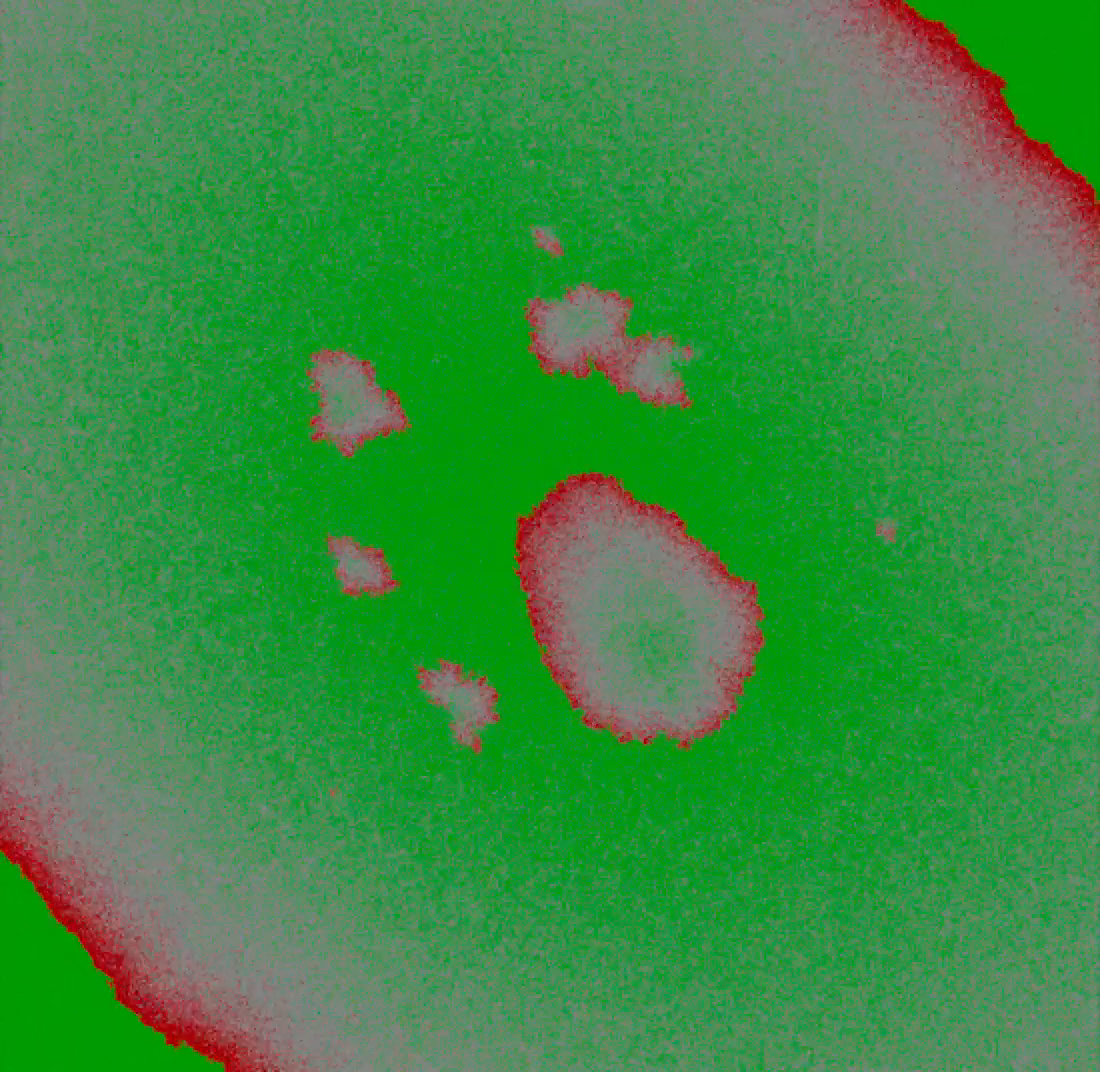
\includegraphics[width = 0.2\textwidth]{../images/predator_prey_11_by_11_f_1_k_2_i4.png} & 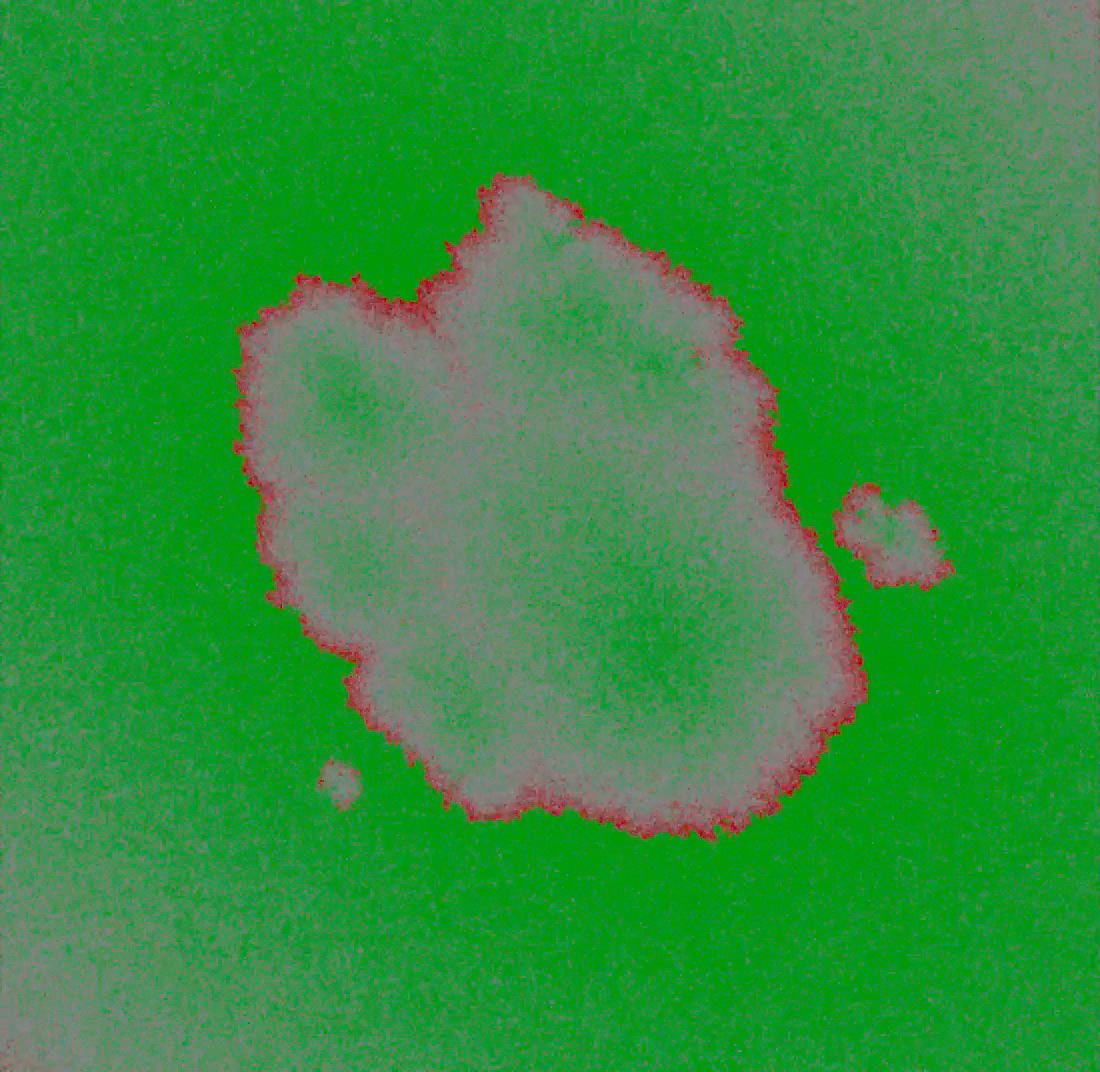
\includegraphics[width = 0.2\textwidth]{../images/../images/predator_prey_11_by_11_f_1_k_2_i5.png} & 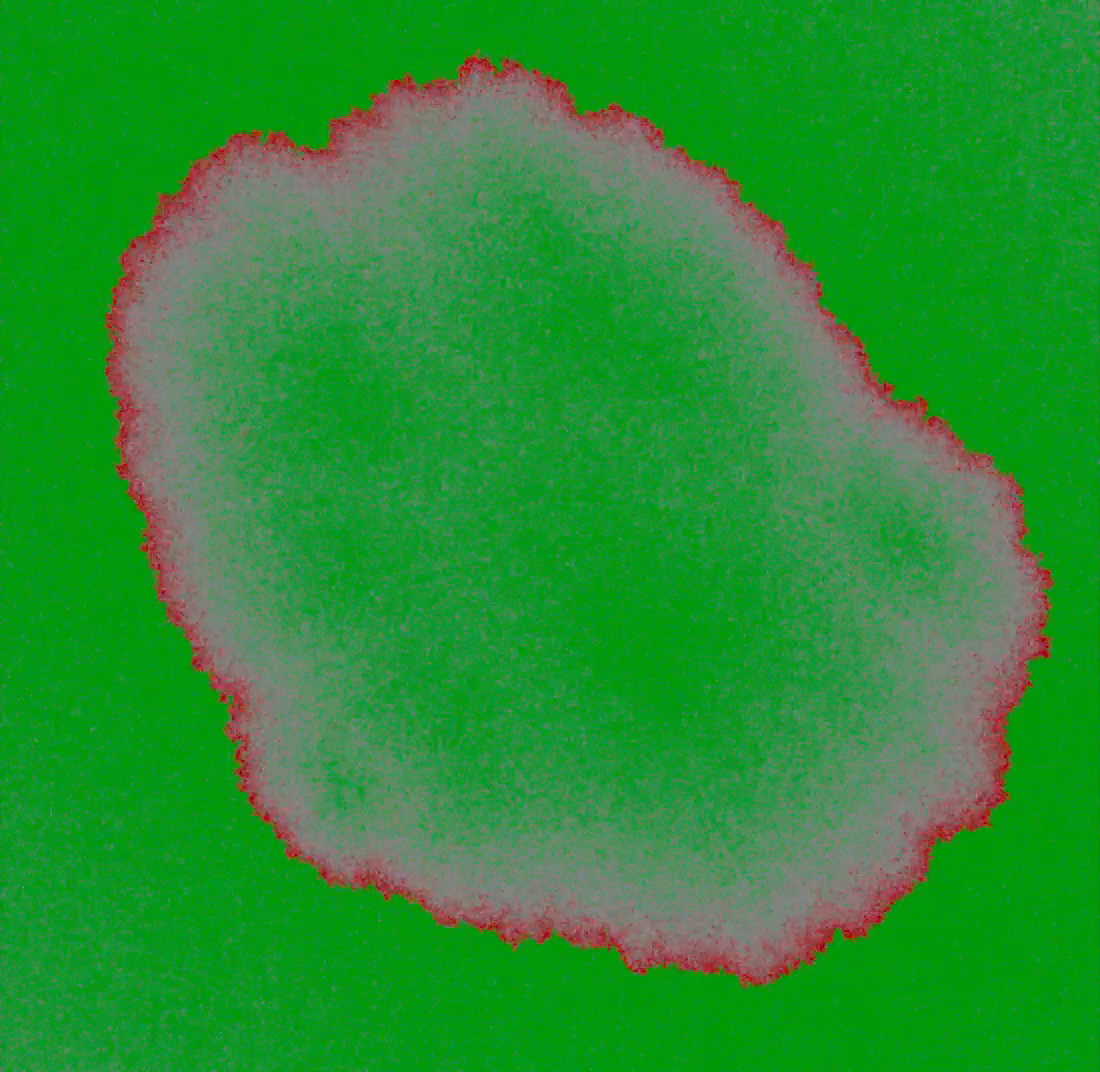
\includegraphics[width = 0.2\textwidth]{../images/../images/predator_prey_11_by_11_f_1_k_2_i6.png} & 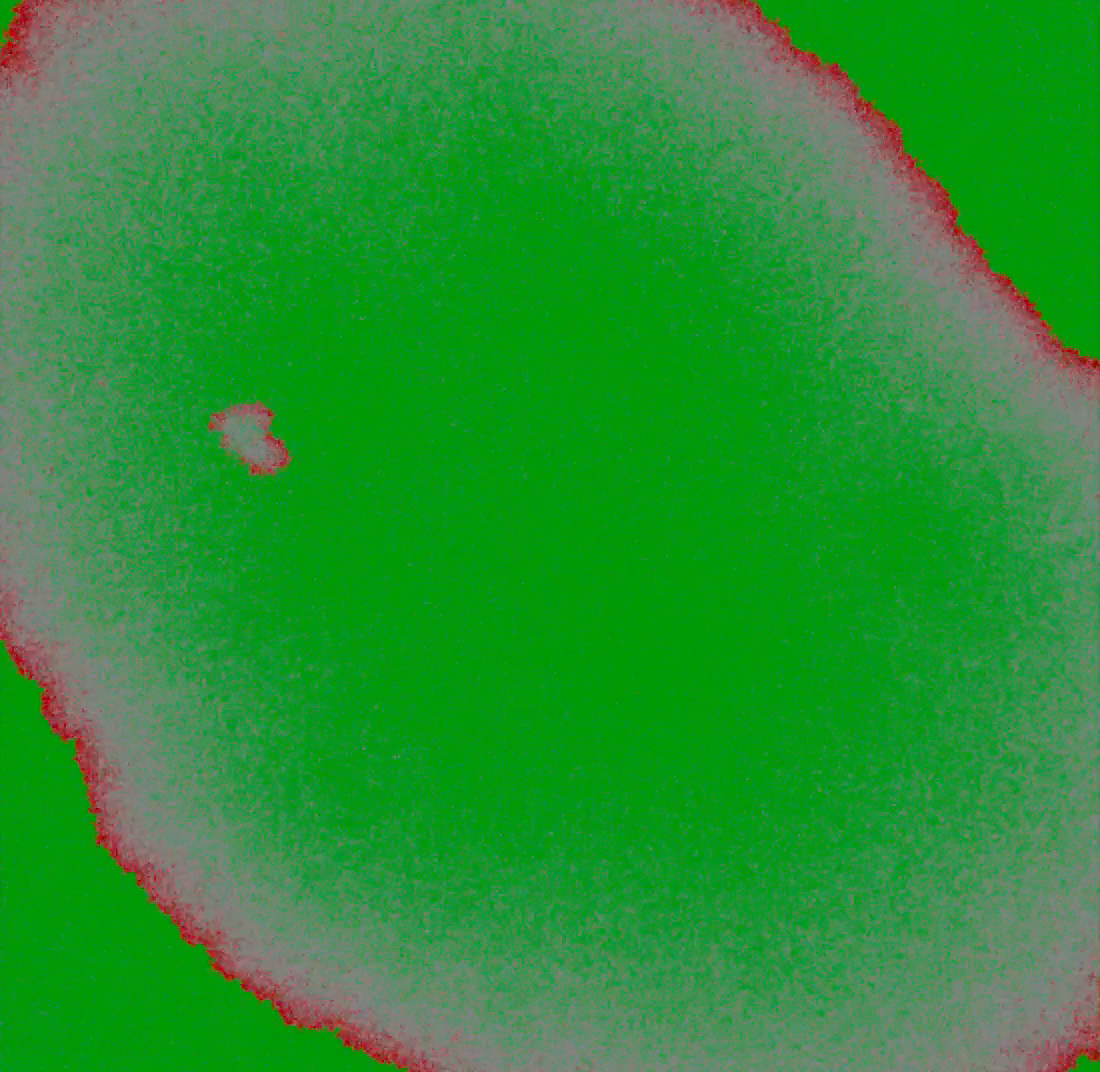
\includegraphics[width = 0.2\textwidth]{../images/../images/predator_prey_11_by_11_f_1_k_2_i7.png}
\end{tabular}
\caption{An animation of a CellBlender simulation of our reaction-diffusion system using the parameter rates \textvar{f} = 100,000 and \textvar{k} = 200,000. For these ``sweet spot'' parameters, we see expanding stripes of \textvar{B} particles.}
\label{fig:k=200000_f=100000}
\end{figure}

When we hold \textvar{k} fixed and start to increase \textvar{f}, the higher feed rate increases the likelihood of \textvar{B} particles encountering \textvar{A} particles, and so we see even more stripes of \textvar{B} particles (\autoref{fig:k=200000_f=140000}).

\begin{figure}[h]
\centering
\mySfFamily
\begin{tabular}{c c c c}

\includegraphics[width = 0.2\textwidth]{../images/predator_prey_11_by_11_f_1.4_k_2.png} & 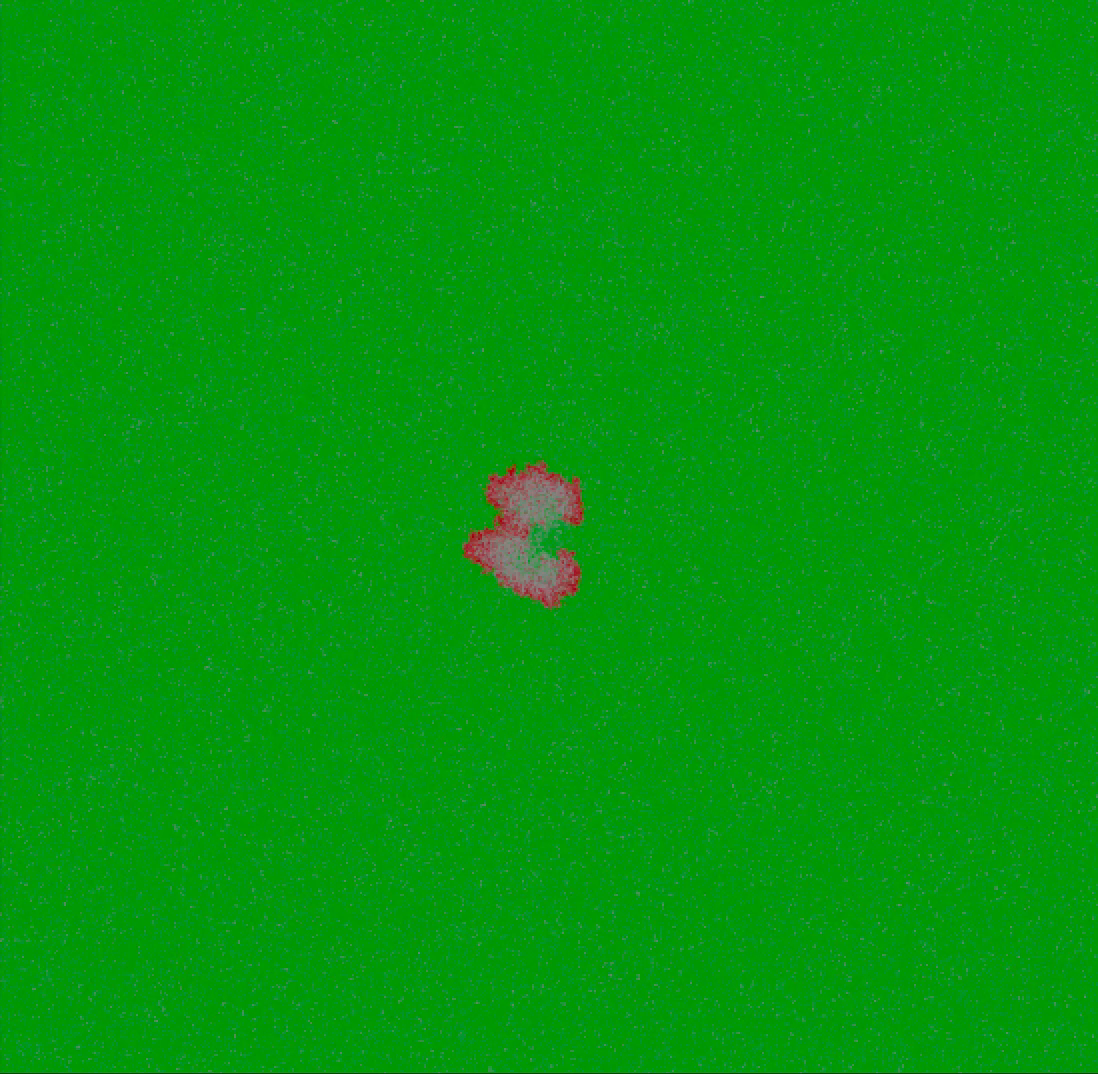
\includegraphics[width = 0.2\textwidth]{../images/../images/predator_prey_11_by_11_f_1.4_k_2_i1.png} & 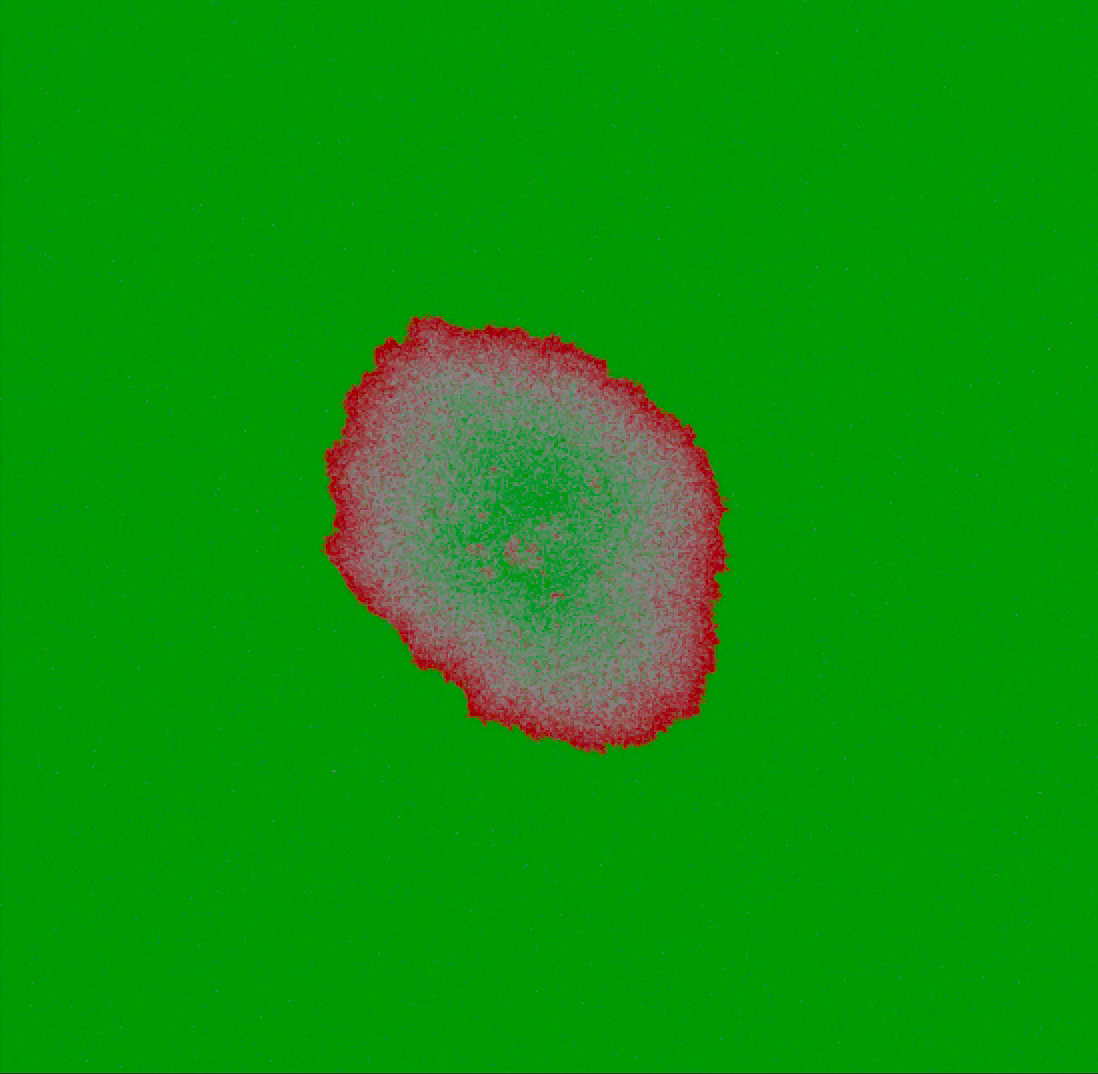
\includegraphics[width = 0.2\textwidth]{../images/../images/predator_prey_11_by_11_f_1.4_k_2_i2.png} & 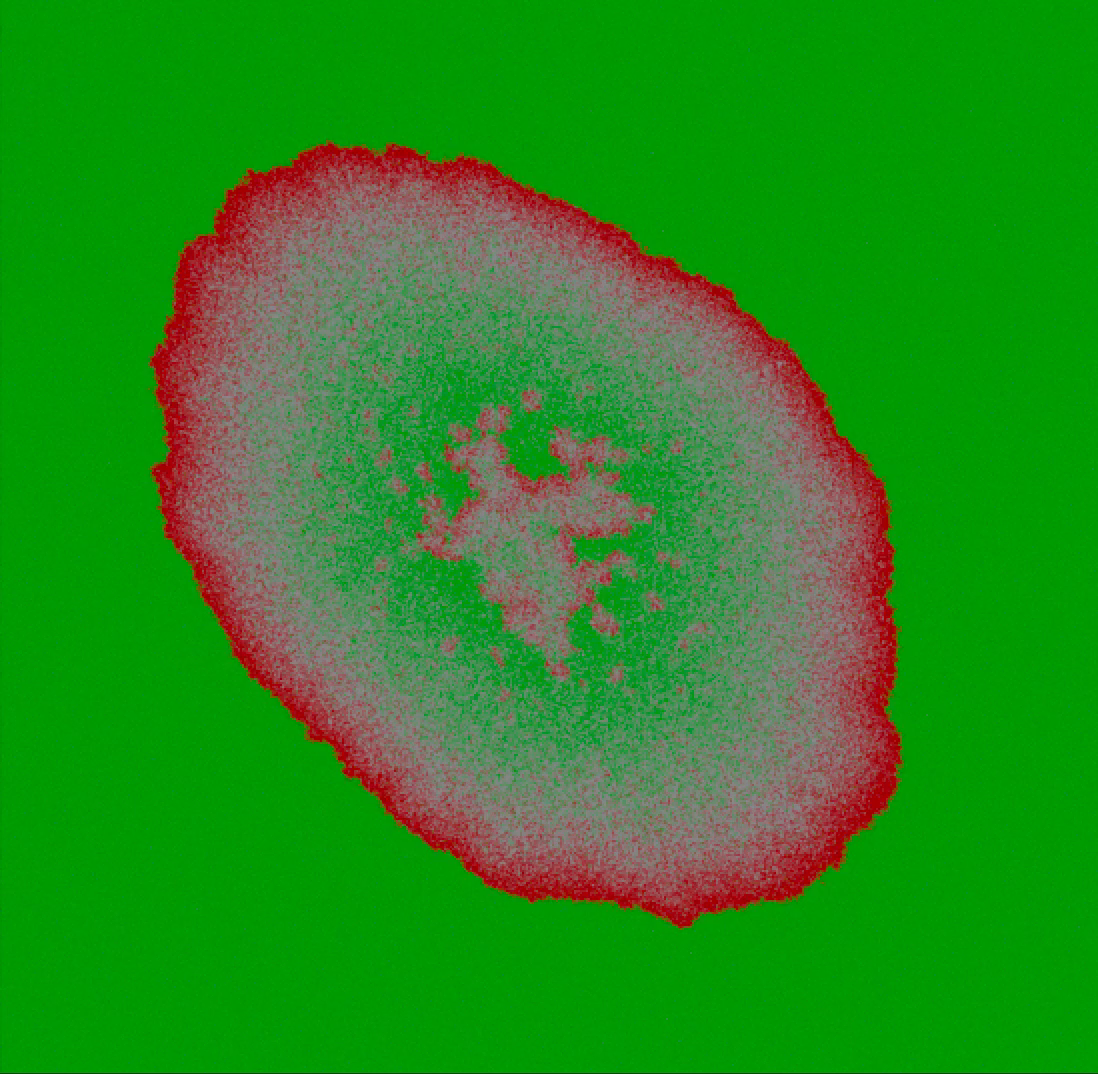
\includegraphics[width = 0.2\textwidth]{../images/../images/predator_prey_11_by_11_f_1.4_k_2_i3.png}\\[2ex]
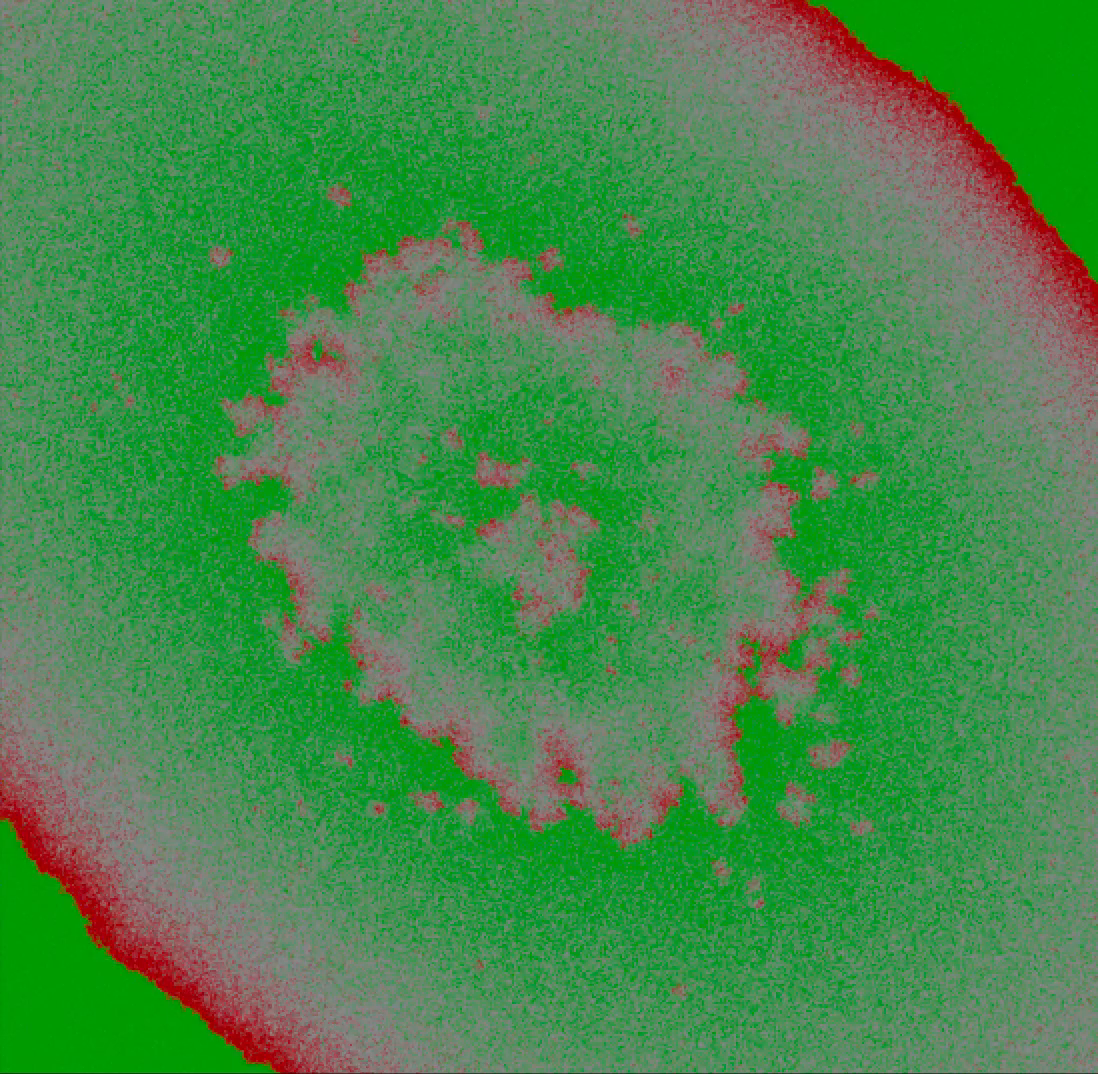
\includegraphics[width = 0.2\textwidth]{../images/predator_prey_11_by_11_f_1.4_k_2_i4.png} & 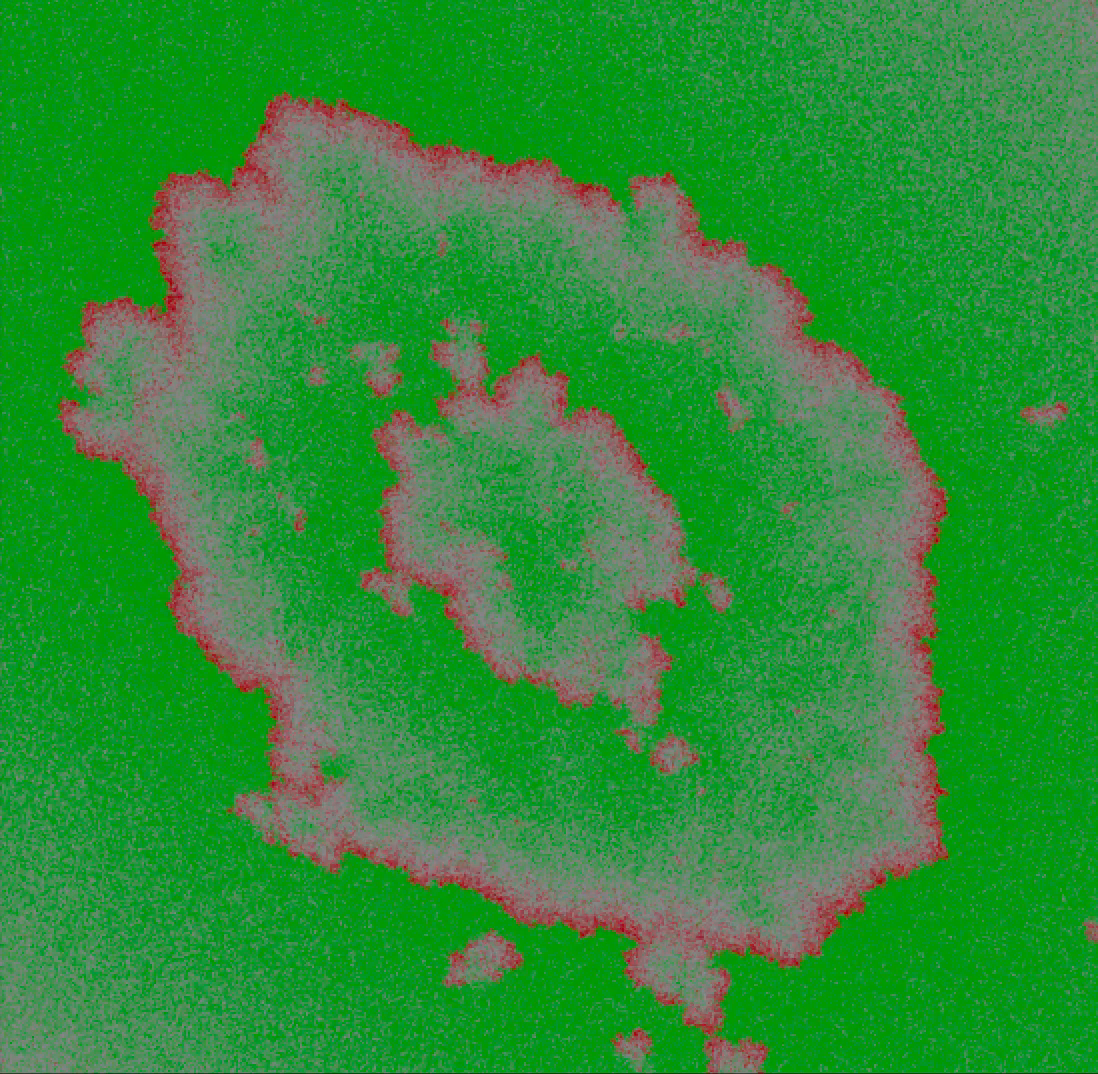
\includegraphics[width = 0.2\textwidth]{../images/../images/predator_prey_11_by_11_f_1.4_k_2_i5.png} & 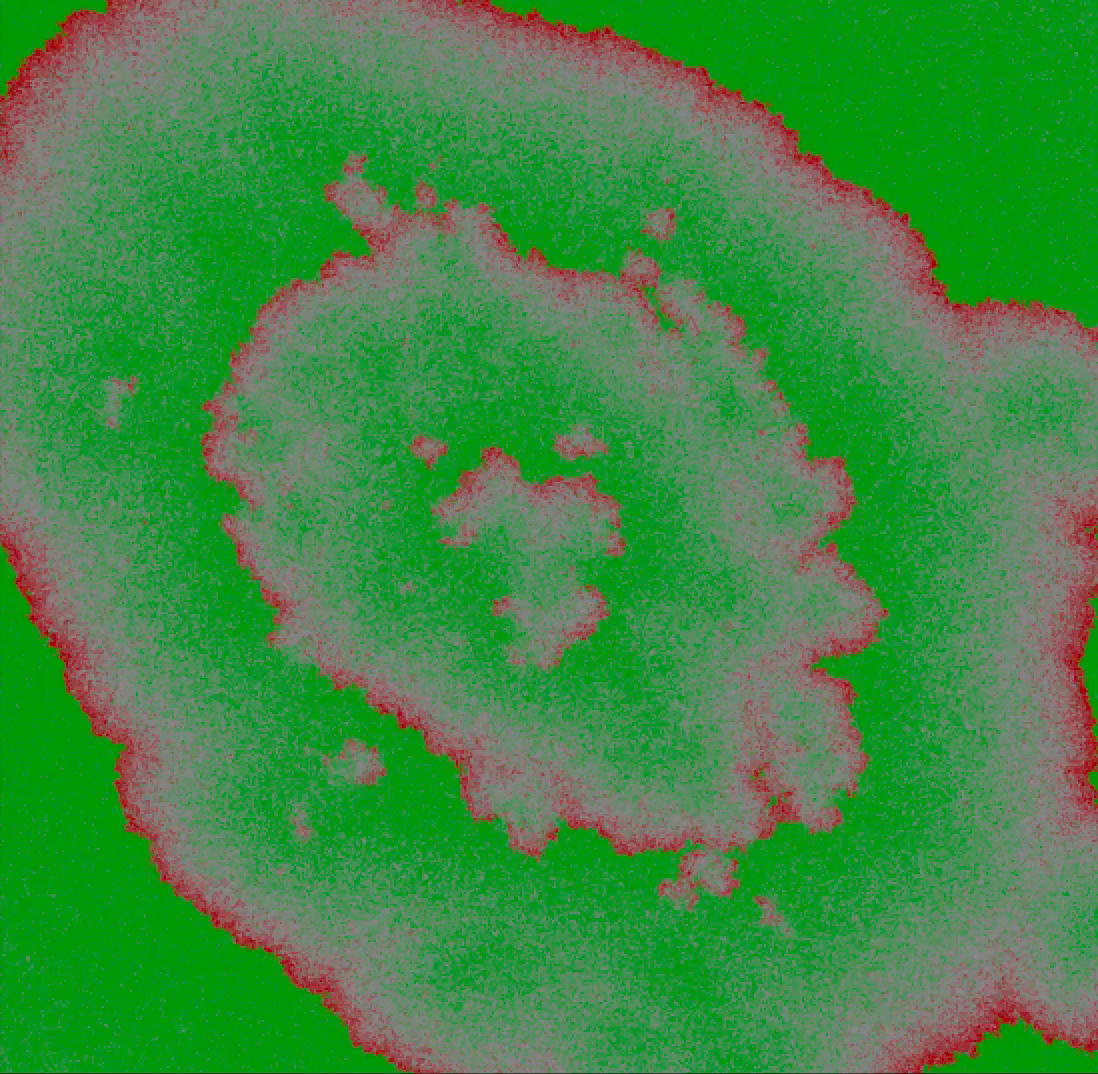
\includegraphics[width = 0.2\textwidth]{../images/../images/predator_prey_11_by_11_f_1.4_k_2_i6.png} & 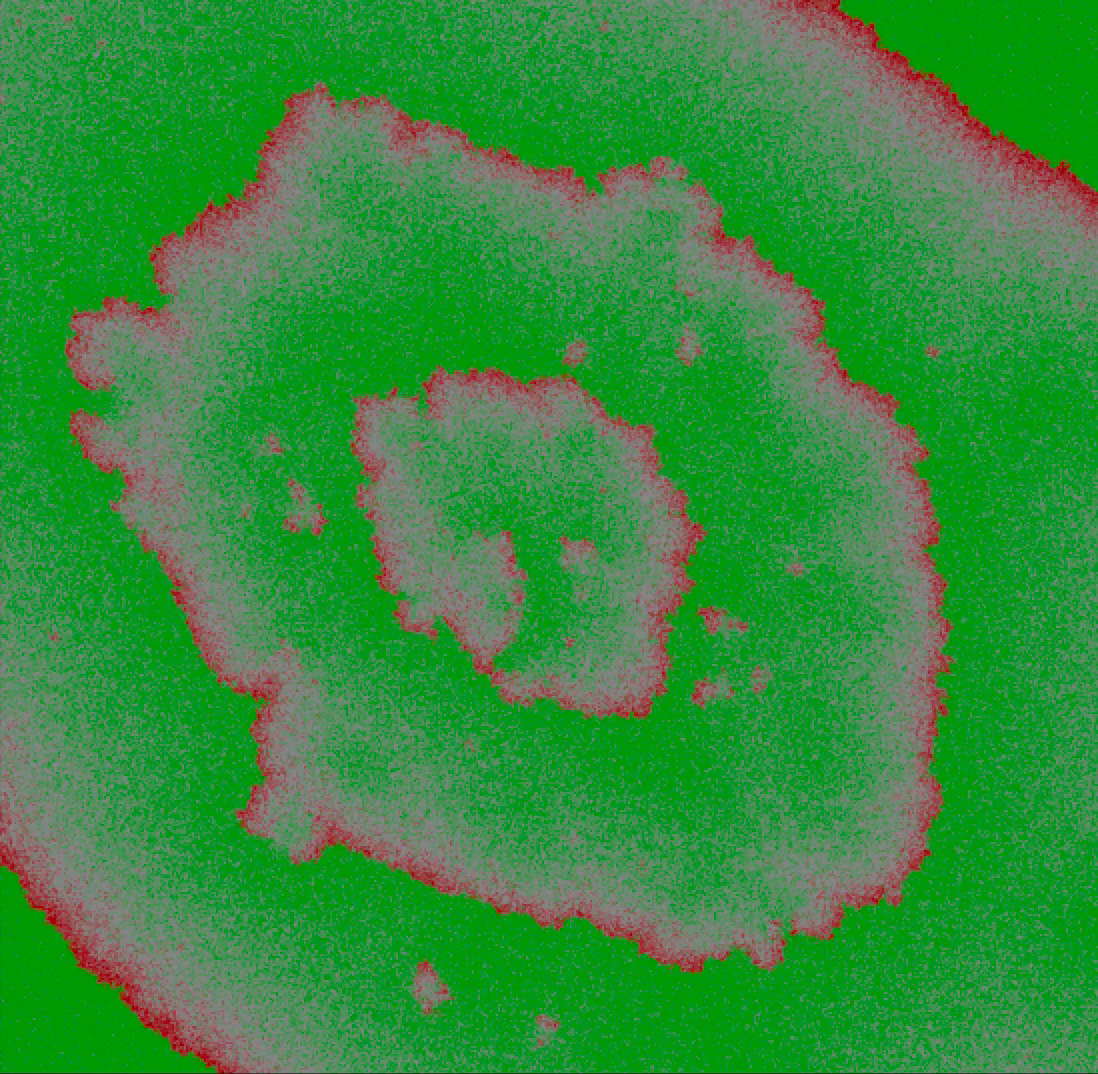
\includegraphics[width = 0.2\textwidth]{../images/../images/predator_prey_11_by_11_f_1.4_k_2_i7.png}
\end{tabular}
\caption{An animation of a CellBlender simulation of our reaction-diffusion system using the parameter rates \textvar{f} = 140,000 and \textvar{k} = 200,000. Because \textvar{f} has increased relative to \textvar{k} compared to \autoref{fig:k=200000_f=100000}, we see even more stripes of \textvar{B} particles.}
\label{fig:k=200000_f=140000}
\end{figure}

As \textvar{f} continues to increase, the stripe structure becomes chaotic and breaks down because there are now many clusters of \textvar{B} particles colliding and mix with each other (\autoref{fig:k=200000_f=175000}).

\begin{figure}[h]
\centering
\mySfFamily
\begin{tabular}{c c c c}
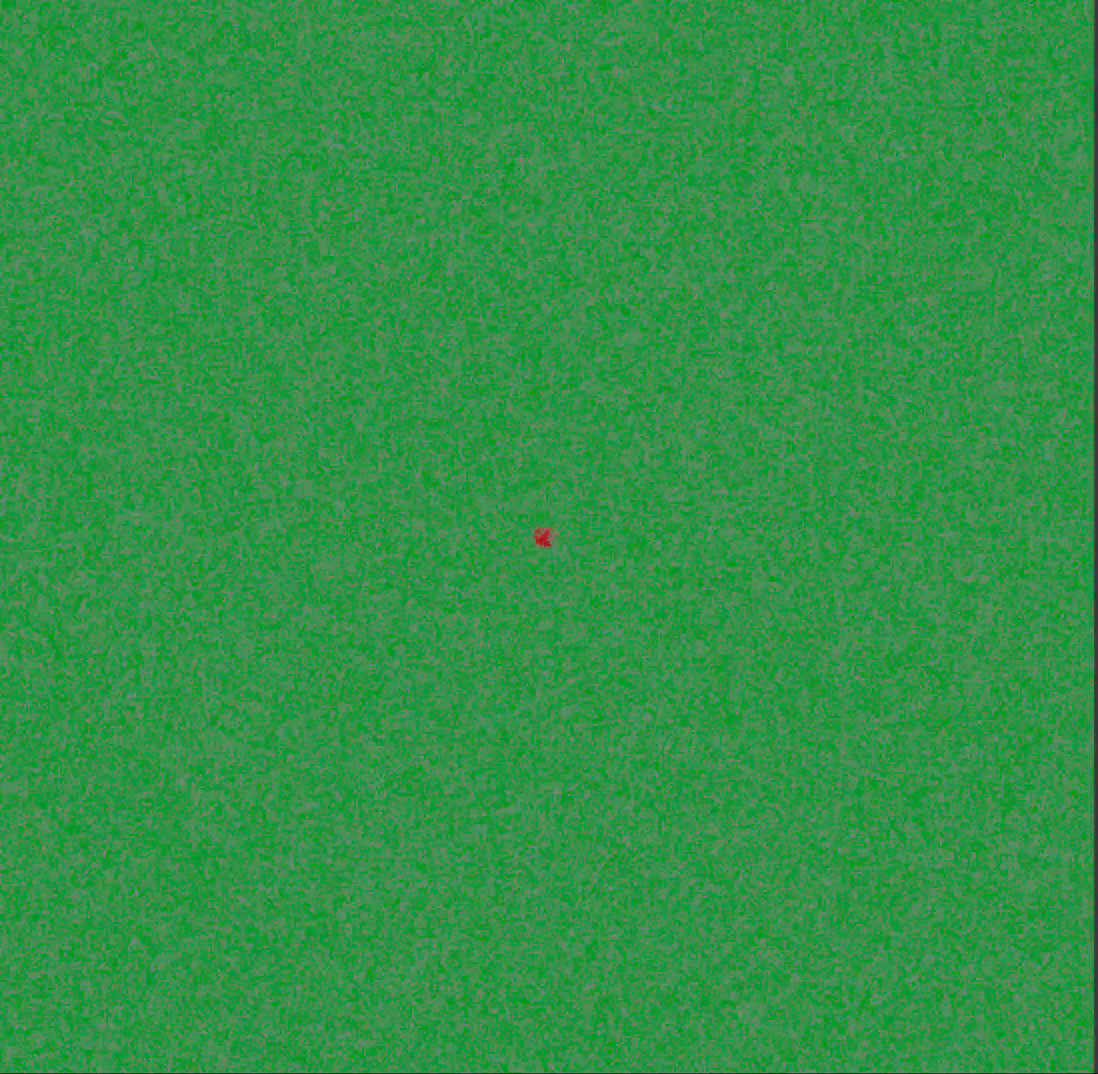
\includegraphics[width = 0.2\textwidth]{../images/predator_prey_11_by_11_f_1.75_k_2_new.png} & 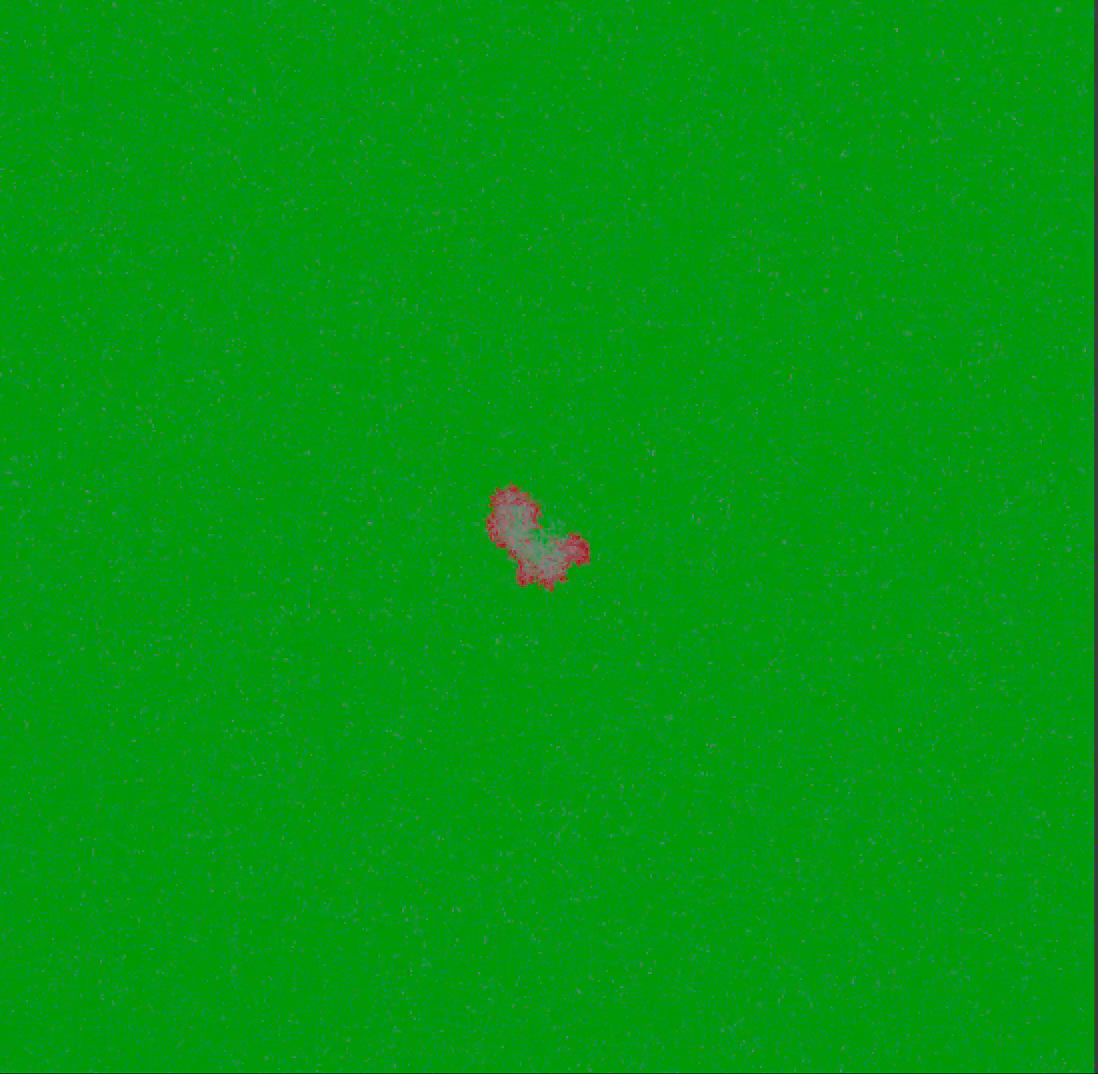
\includegraphics[width = 0.2\textwidth]{../images/../images/predator_prey_11_by_11_f_1.75_k_2_new_i1.png} & 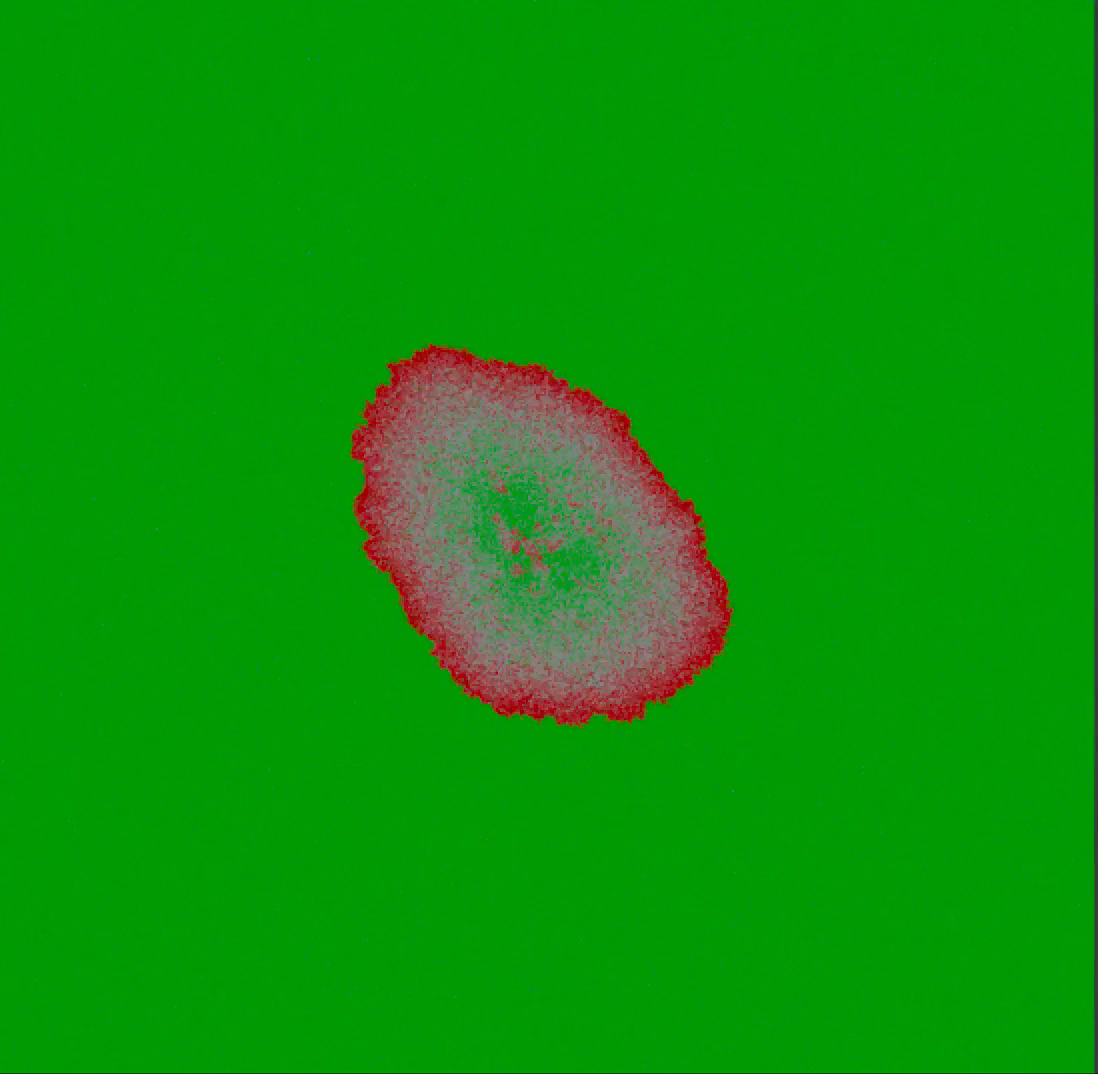
\includegraphics[width = 0.2\textwidth]{../images/../images/predator_prey_11_by_11_f_1.75_k_2_new_i2.png} & 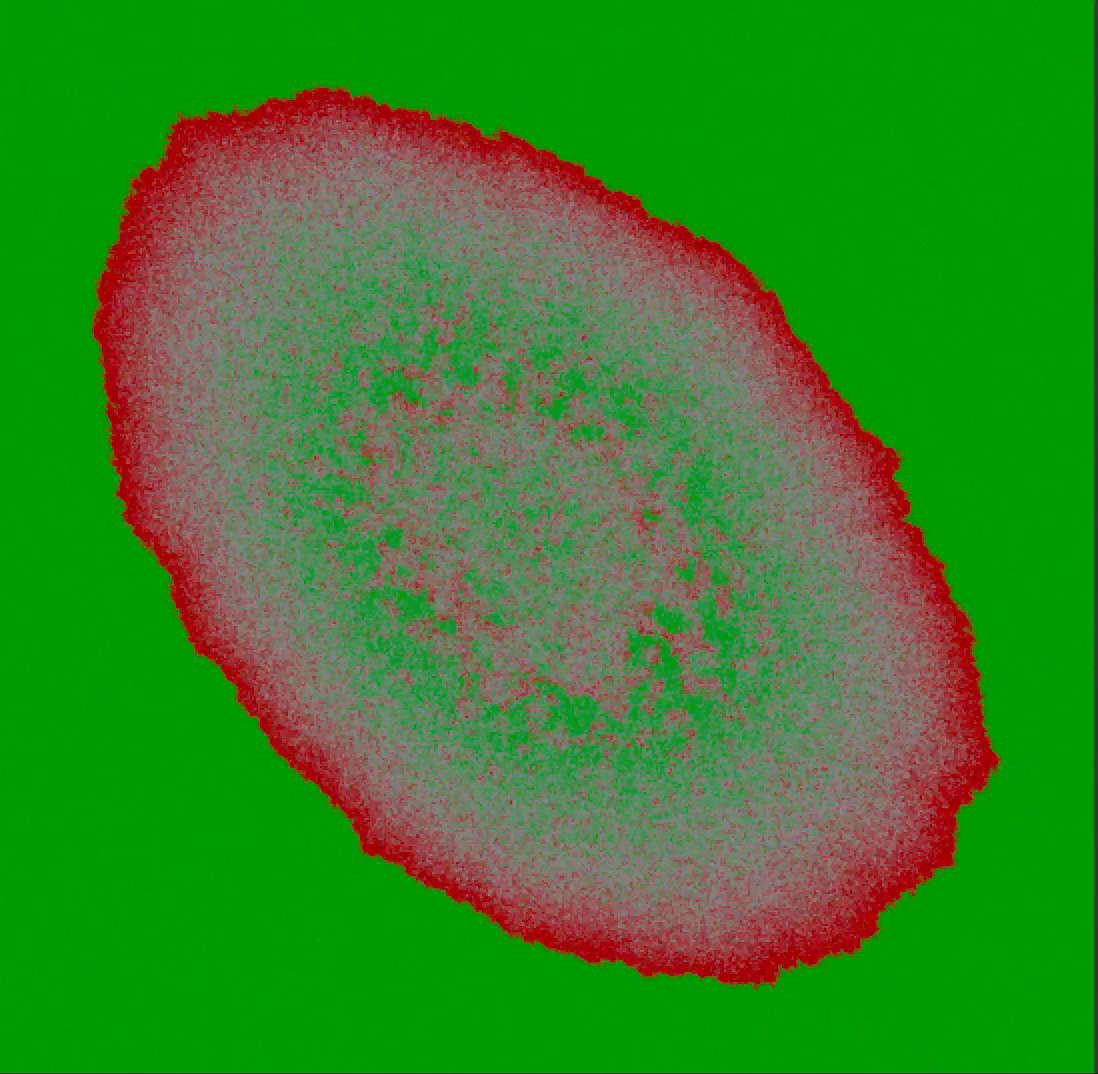
\includegraphics[width = 0.2\textwidth]{../images/../images/predator_prey_11_by_11_f_1.75_k_2_new_i3.png}\\[2ex]
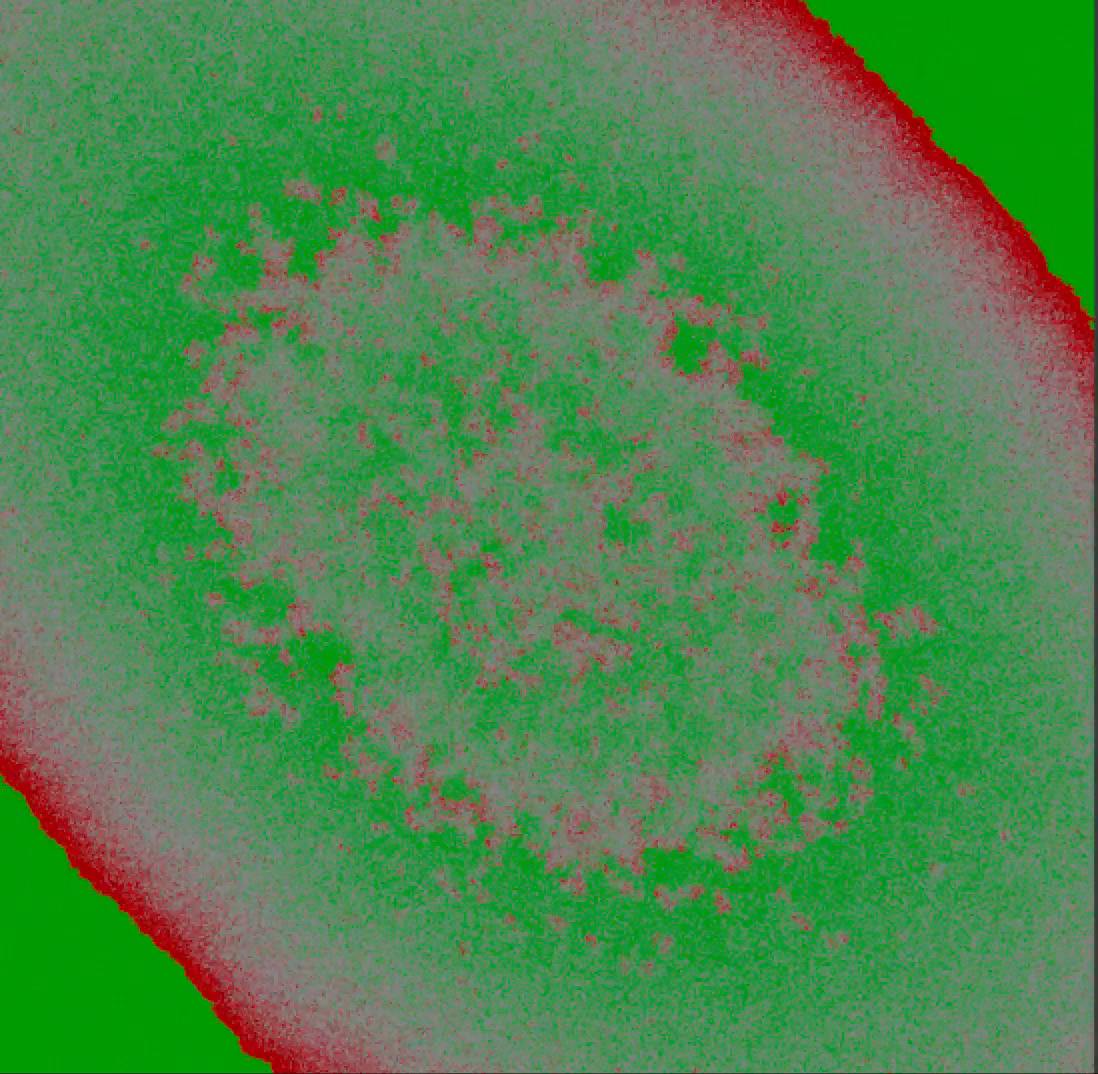
\includegraphics[width = 0.2\textwidth]{../images/predator_prey_11_by_11_f_1.75_k_2_new_i4.png} & 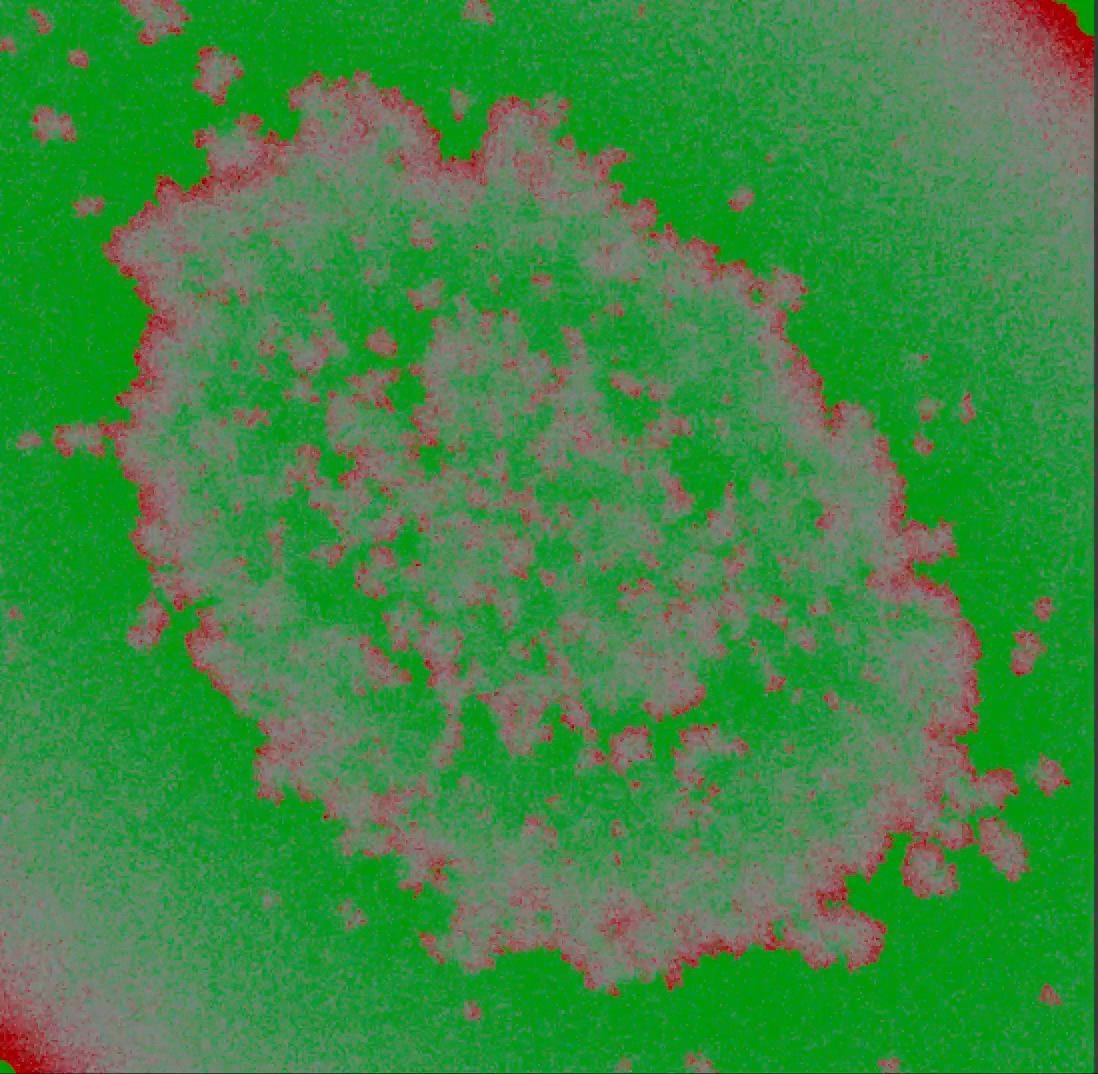
\includegraphics[width = 0.2\textwidth]{../images/../images/predator_prey_11_by_11_f_1.75_k_2_new_i5.png} & 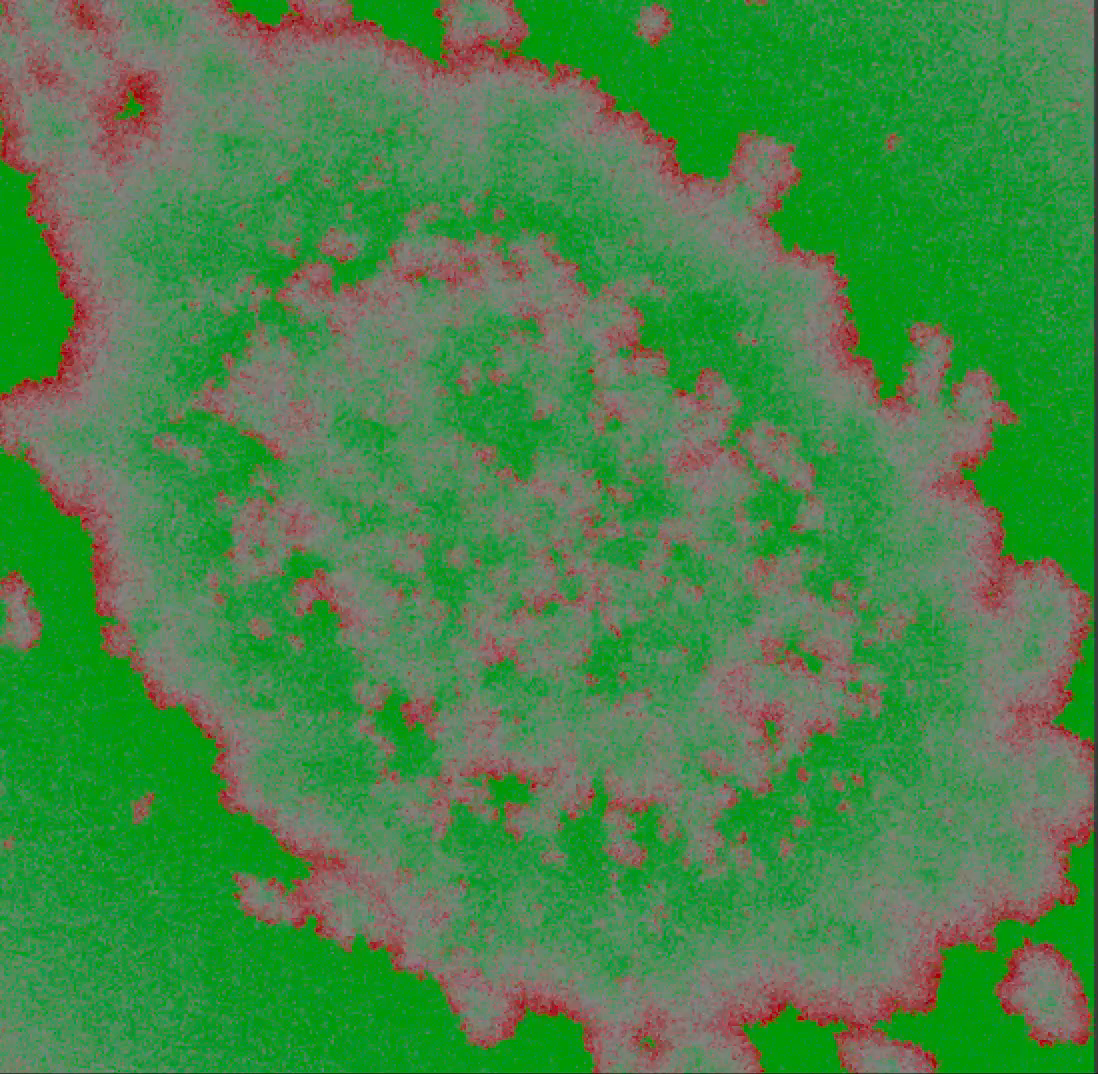
\includegraphics[width = 0.2\textwidth]{../images/../images/predator_prey_11_by_11_f_1.75_k_2_new_i6.png} & 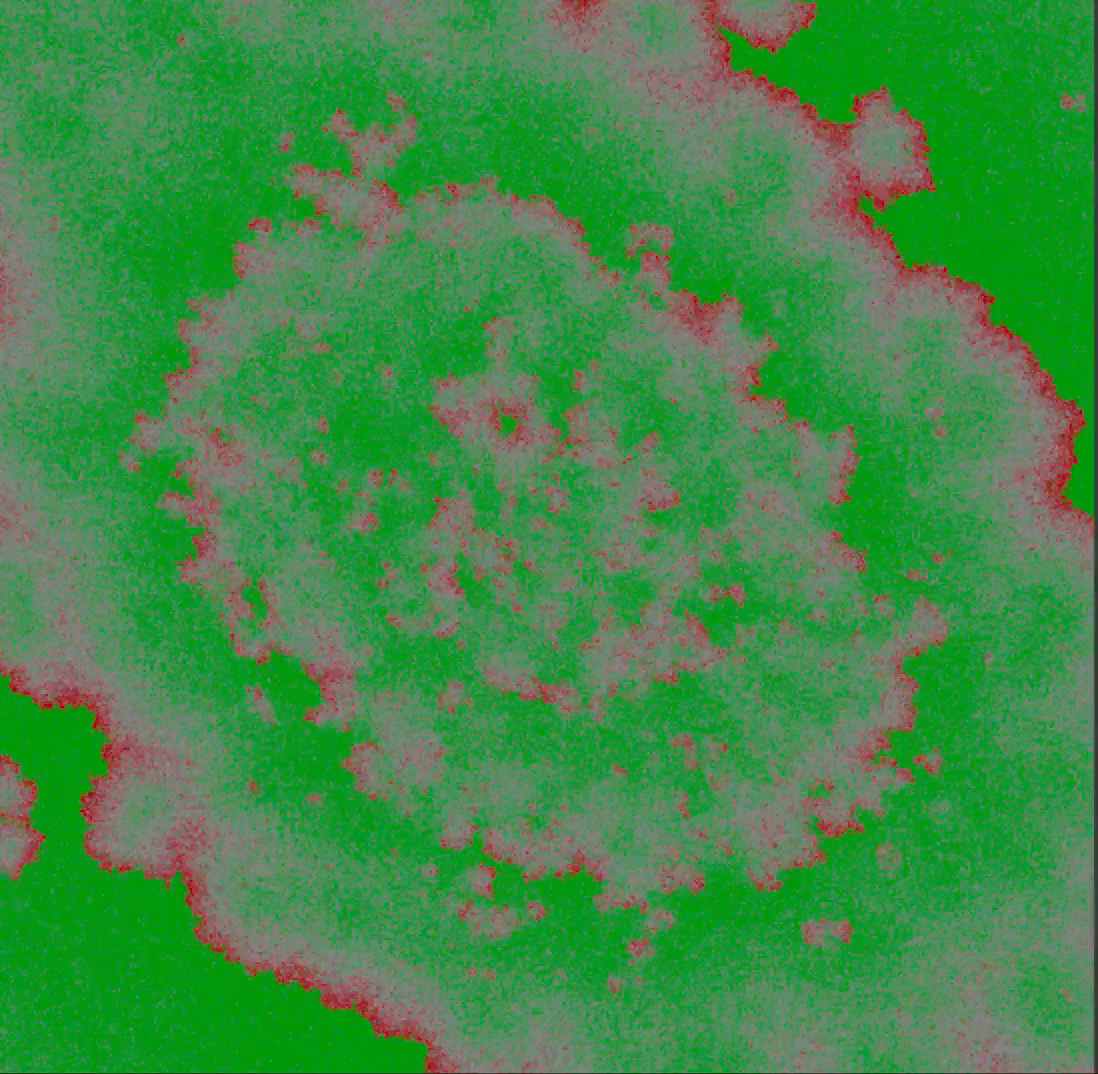
\includegraphics[width = 0.2\textwidth]{../images/../images/predator_prey_11_by_11_f_1.75_k_2_new_i7.png}
\end{tabular}
\caption{An animation of a CellBlender simulation of our reaction-diffusion system using the parameter rates \textvar{f} = 175,000 and \textvar{k} = 200,000. There are so many pockets of \textvar{B} particles that the stripe patterns start to break down.}
\label{fig:k=200000_f=175000}
\end{figure}

A subsequent increase in \textvar{f} causes the stripes to disappear (\autoref{fig:k=100000_f=100000}). We might expect this to mean that the \textvar{A} and \textvar{B} particles will be uniformly mixed. Instead, we see that after an initial outward explosion of \textvar{B} particles, the system displays a \textit{mottled} background, with clusters having higher or lower concentration of \textvar{B}. Patterns in the simulation are noisy --- even in the dark red regions we will have quite a few green particles, and vice-versa. The rapid inference of large-scale patterns from small-scale visual phenomena is one of the tasks that our brains have evolved to perform well.

\begin{figure}[h]
\centering
\mySfFamily
\begin{tabular}{c c c c}
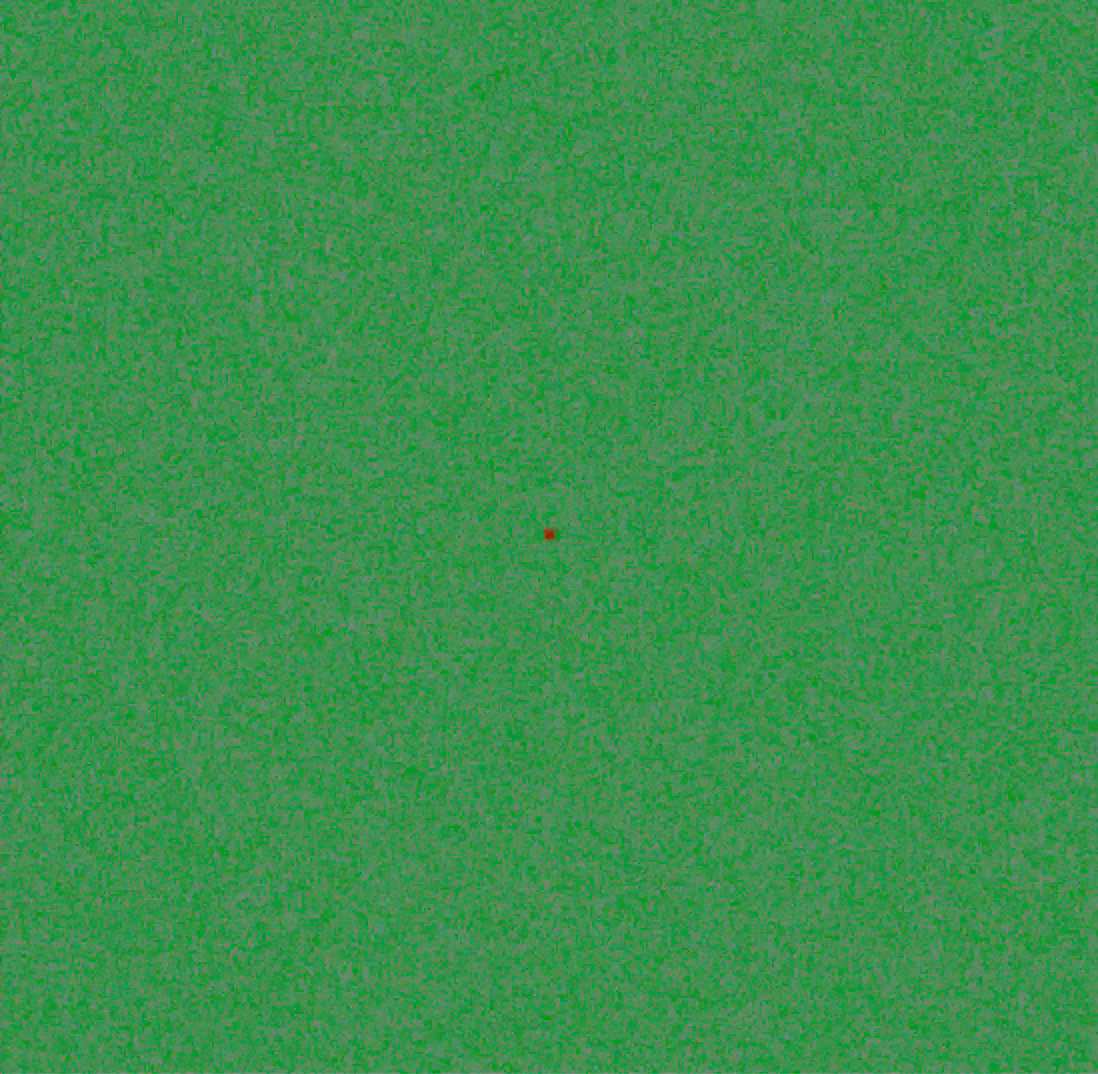
\includegraphics[width = 0.2\textwidth]{../images/predator_prey_11_by_11_f_1_k_1.png} & 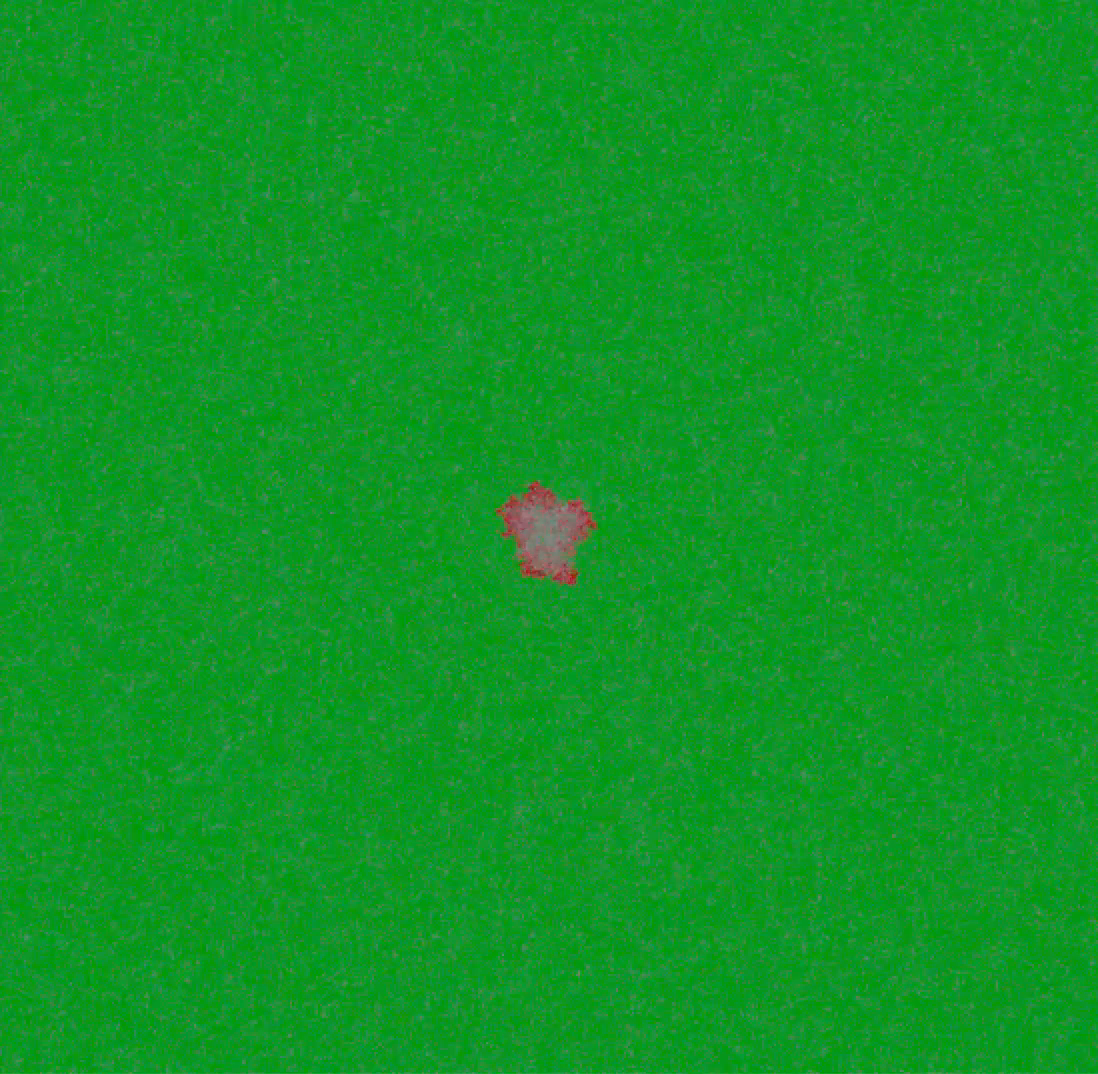
\includegraphics[width = 0.2\textwidth]{../images/../images/predator_prey_11_by_11_f_1_k_1_i1.png} & 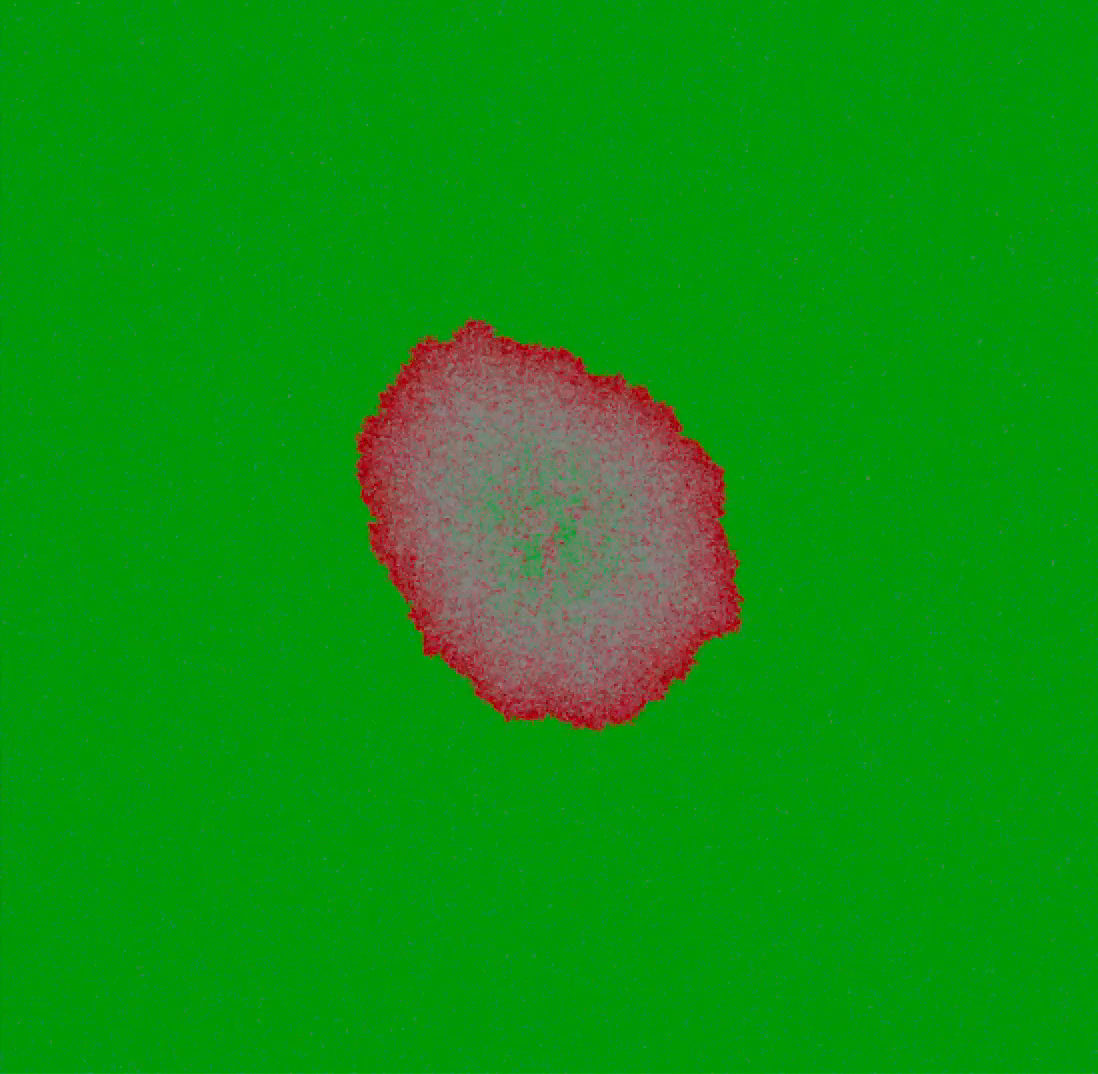
\includegraphics[width = 0.2\textwidth]{../images/../images/predator_prey_11_by_11_f_1_k_1_i2.png} & 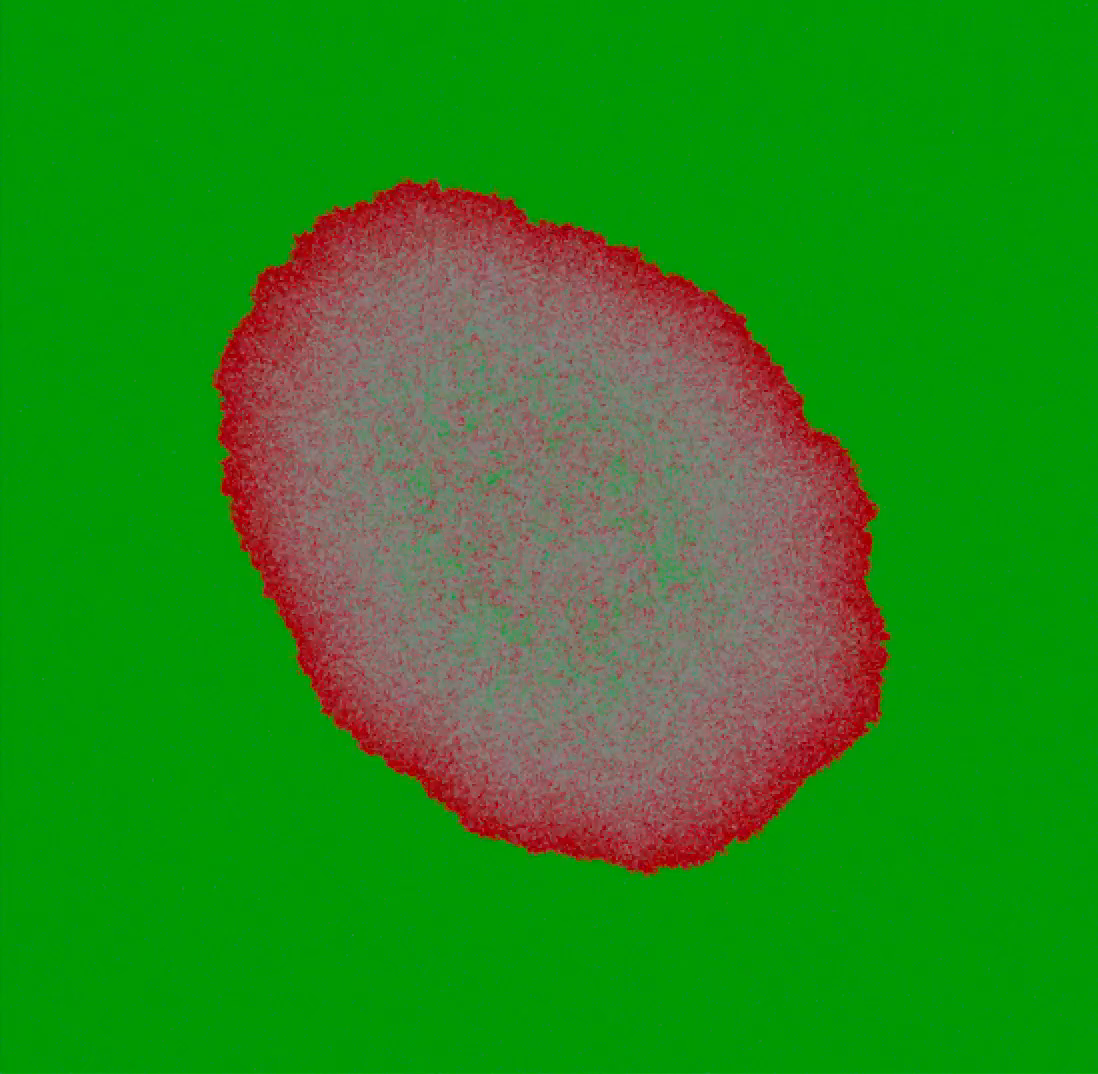
\includegraphics[width = 0.2\textwidth]{../images/../images/predator_prey_11_by_11_f_1_k_1_i3.png}\\[2ex]
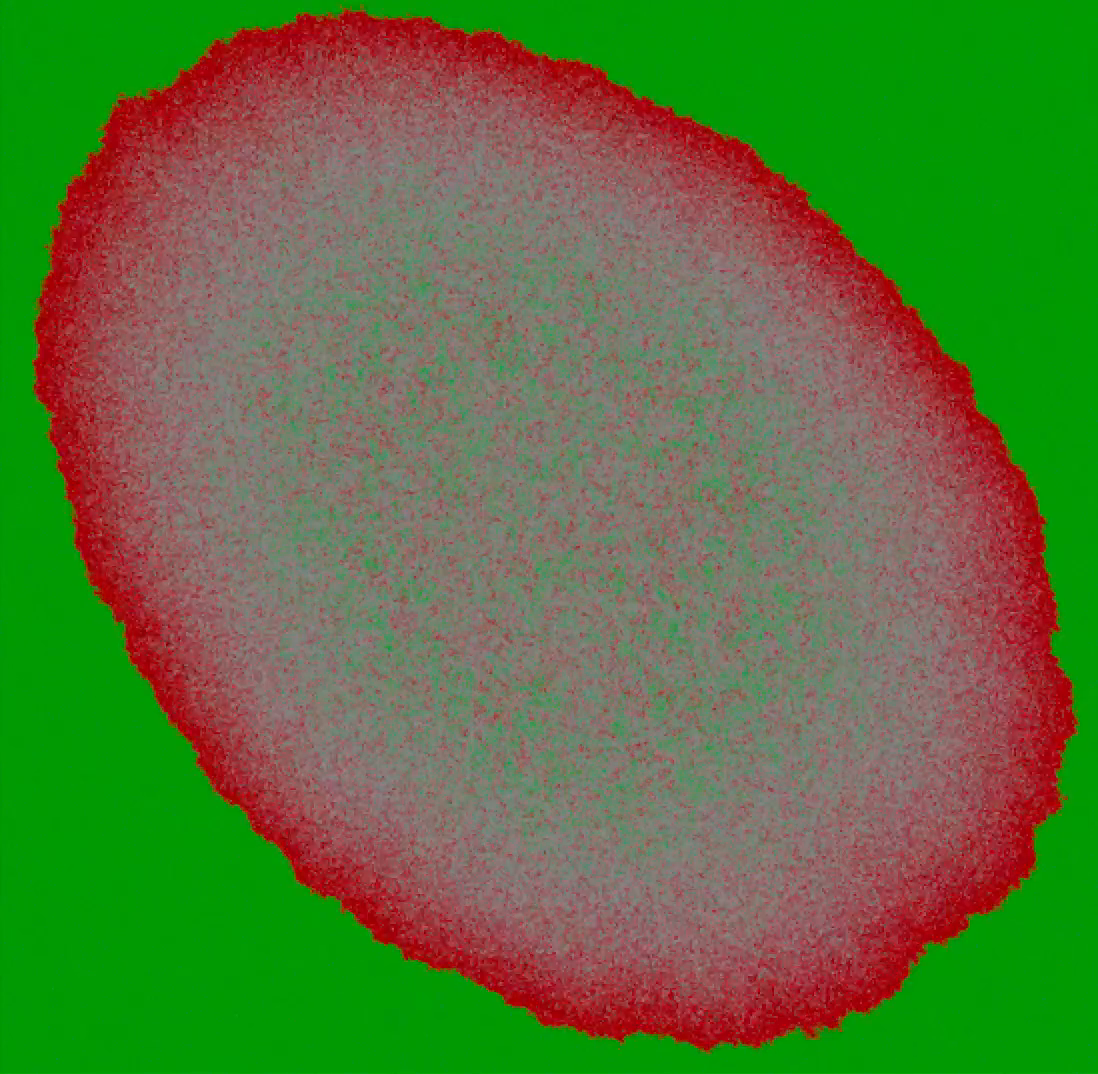
\includegraphics[width = 0.2\textwidth]{../images/predator_prey_11_by_11_f_1_k_1_i4.png} & \includegraphics[width = 0.2\textwidth]{../images/../images/predator_prey_11_by_11_f_1_k_1_i5.png} & \includegraphics[width = 0.2\textwidth]{../images/../images/predator_prey_11_by_11_f_1_k_1_i6.png} & \includegraphics[width = 0.2\textwidth]{../images/../images/predator_prey_11_by_11_f_1_k_1_i7.png}
\end{tabular}
\caption{An animation of a CellBlender simulation of our reaction-diffusion system using the parameter rates \textvar{f} = 100,000 and \textvar{k} = 100,000. Now that the feed rate is equal to the kill rate, after an initial wave of \textvar{B} particles, the \textvar{B} particles form so many clusters that they produce a mottling effect.}
\label{fig:k=100000_f=100000}
\end{figure}

You may still be skeptical, since the patterns in these figures do not have the concrete boundaries that we might expect of animal stripes and spots. Yet when we closely examine an animal with skin patterns, we can see that, like a pointillist painting, the patterns we infer on a higher level are just the net result of varied individual points (\autoref{fig:zebrafish_zoom}).\\

\begin{figure}[h]
\centering
\mySfFamily
\includegraphics[width = 0.6\textwidth]{../images/zebrafish_zoom.jpg}
\caption{Zooming in on the striped skin of a zebrafish shows that each stripe is formed of many differently colored cells, and that the boundaries of the stripes are more variable than they may seem at lower resolution.}
\label{fig:zebrafish_zoom}
\end{figure}

\FloatBarrier
\phantomsection
\subsection{Turing's patterns and Klüver's form constants}

The particle simulations in the previous subsection may evoke the adjective ``trippy''. This is no accident.

Research dating to the 1920s has studied the patterns that we see during visual hallucinations, which Heinrich Klüver named \textdef{form constants}{form constants}{patterns seen during visual hallucinations, which recur across patients and were first studied by Heinrich Klüver in the 1920s} after studying patients who had taken mescaline. Form constants, such as cobwebs, tunnels, and spirals, occur across many individuals, regardless of the cause of their hallucinations (\autoref{fig:form_constants}).\\

\begin{figure}[h]
\centering
\mySfFamily
\includegraphics[width = 0.6\textwidth]{../images/form_constants.png}
\caption{A few of Heinrich Klüver's form constants.}
\label{fig:form_constants}
\end{figure}

Over five decades after Klüver's work, researchers would determine that form constants having different shapes originate from simpler \textit{linear} stripes of cellular activation patterns in the retina. The retina is circular, but the brain needs to convert this cellular image into a rectangular field of view; as a result, when the linear patterns are passed to the visual cortex, the hallucinating brain contorts them into the spirals and whirls that we see. Some researchers believe that the patterns in the retina caused by hallucinations are in fact Turing patterns and can be explained by a reaction-diffusion model in which one type of neuron acts as a predator and another acts as prey.\\

\FloatBarrier
\phantomsection
\section{A Coarse-Grained Model of Particle Diffusion}
\label{sec:coarse_grained_diffusion}

\phantomsection
\subsection{Diffusion of a single particle}

Despite using advanced modeling software that has undergone years of development and optimization, each of the simulations in the previous section took several hours to render. Part of a modeler's job is to find simple models that capture the essence of a system while running quickly and scaling well to larger inputs. Is there a simplifying speed-up that we can make to our model that will still produce Turing patterns?

We have a very ``fine-grained'' reaction-diffusion model illustrating Turing patterns, but this model consumes a huge amount of computational resources because it requires tracking the movements of hundreds of thousands of individual particles. Our goal is to build a ``coarse-grained'' model that will allow us to appreciate Turing patterns without the computational overhead required to track particles.

Our idea is to grid off two-dimensional space into blocks and store only the \textit{concentration} of each type of particle found inside the block. To simplify things further, we assume that there is some maximum concentration of particles possible, so that we can divide the number of particles by this maximum concentration. As a result, the concentration of a particle in each block will be represented by a decimal number between 0 and 1.

Let us begin with an example of the diffusion of only \textvar{A} particles; we will later add \textvar{B} particles as well as reactions to our model. Say that the particles are at maximum concentration in the central cell of our grid and are present nowhere else (\autoref{fig:initial_A_concentration_one_time_step} (left)).

\begin{figure}[h]
\centering
\mySfFamily
\tabcolsep = 2em
\begin{tabular}{c c}
\includegraphics[width = 0.35\textwidth]{../images/initial_A_concentration.png} & \includegraphics[width = 0.35\textwidth]{../images/A_concentration_one_time_step.png}
\end{tabular}
\caption{(Left) A $\text{5} \times \text{5}$ grid showing hypothetical initial concentrations of \textvar{A} particles. Cells are labeled by numbers between 0 and 1 representing their concentration of \textvar{A} particles. The central cell has maximum concentration, and no particles are contained in any other cell. (Right) An updated grid following diffusion of particles after a single time step.}
\label{fig:initial_A_concentration_one_time_step}
\end{figure}

We will now update the grid of cells after one time step to mimic particle diffusion. To do so, we will spread out the concentration of particles in each square to its eight neighbors. For example, we could assume that 20\% of the current cell's concentration diffuses to each of its four adjacent neighbors, and that 5\% of the cell's concentration diffuses to its four diagonal neighbors. Because the central square in our ongoing example is the only cell with any particles, only its neighbors will receive any particles after a single time step (\autoref{fig:initial_A_concentration_one_time_step} (right)).\\

\begin{note}[%
The sum of the values in each grid in \autoref{fig:initial_A_concentration_one_time_step} is 1. Regardless of how many times we update the grid, the sum of the values should be 1 to ensure the conservation of total mass in the system.
]\end{note}

After an additional time step (\autoref{fig:A_concentration_two_time_steps_partial}), the particles continue to diffuse outward. For example, each diagonal neighbor of the central cell in the above figure, which has a concentration of 0.05 after one time step, will lose all of its particles in the following step. Each of these cells will also gain 20\% of the particles from two of its adjacent neighbors, along with 5\% of the particles from the central square (which doesn't have any particles). This makes the updated concentration of this cell after two time steps equal to $2 \cdot 0.2 \cdot 0.2 + 0.05 \cdot 0 = 0.08$.

The four cells directly adjacent to the central square, which have a concentration of 0.2 after one time step, will also gain particles from their neighbors. Each such cell will receive 20\% of the particles from two of its adjacent neighbors and 5\% of the particles from two of its diagonal neighbors, which have a concentration of 0.2. Therefore, the updated concentration of each of these cells after two time steps is $2 \cdot 0.2 \cdot 0.05 + 2 \cdot 0.05 \cdot 0.2 = 0.04$.

Finally, the central square has no particles after one step, but it will receive 20\% of the particles from each of its four adjacent neighbors, as well as 5\% of the particles from each of its four diagonal neighbors. As a result, the central square's concentration after two time steps is $4 \cdot 0.2 \cdot 0.2 + 4 \cdot 0.05 \cdot 0.05 = 0.16 + 0.01 = 0.17$.\\

\begin{figure}[h]
\centering
\mySfFamily
\includegraphics[width = 0.35\textwidth]{../images/A_concentration_two_time_steps_partial.png}
\caption{A grid showing an update to the central nine squares of the diffusion system in \autoref{fig:initial_A_concentration_one_time_step} after an additional time step. The cells labeled ``?'' are left as an exercise for the reader.}
\label{fig:A_concentration_two_time_steps_partial}
\end{figure}

\begin{qbox}[%
What should the values of the ``?'' cells be in \autoref{fig:A_concentration_two_time_steps_partial}? Note that these cells are neighbors of cells with positive concentrations after one time step, and so their concentrations should be positive after two time steps.
]\end{qbox}

The coarse-grained model of particle diffusion that we have built is a variant of a \textdef{cellular automaton}{cellular automaton}{a grid of cells in which we use fixed rules to update the status of a cell based on its current status and those of its neighbors}, or a grid of cells in which we use fixed rules to update the status of a cell based on its current status and those of its neighbors.\\

\begin{note}[%
Cellular automata form a rich area of research applied to a wide variety of fields dating back to the middle of the 20th Century; if you are interested in learning more about them from the perspective of programming, then you might like to check out the Programming for Lovers project (\url{http://programmingforlovers.com}).
]\end{note}

\FloatBarrier
\phantomsection
\subsection{Slowing down the diffusion rate}

There is just one problem: our cellular automaton model of diffusion is too volatile! In 
\autoref{fig:initial_A_concentration_one_time_step} and \autoref{fig:A_concentration_two_time_steps_partial}, we see that all of the particles rush out of the central cell in the first time step, only for some of them to return in the next step.

Our solution is to slow down the diffusion process by adding a parameter $d_A$ between 0 and 1 that represents the \textit{rate} of diffusion of \textvar{A} particles. Instead of moving a cell's entire concentration of particles to its neighbors in a single time step, we move only a fraction $d_A$ of them.

Revisiting our original example of a single central cell containing a maximum concentration of $A$ particles, say that $d_A$ is equal to 0.2. After the first time step, only 20\% of the central cell's particles will be spread to its neighbors. Of these particles, 5\% will be spread to diagonal neighbors, and 20\% will be spread to adjacent neighbors. \autoref{fig:A_concentration_slower_diffusion} illustrates that after one time step, the central square has concentration 0.8, its adjacent neighbors have concentration $0.2 \cdot d_A = 0.04$, and its diagonal neighbors have concentration $0.05 \cdot d_A = 0.01$.\\

\begin{figure}[h]
\centering
\mySfFamily
\includegraphics[width = 0.35\textwidth]{../images/A_concentration_slower_diffusion.png}
\caption{An updated grid of cells for the initial grid in \autoref{fig:initial_A_concentration_one_time_step} (left) showing the concentration of \textvar{A} particles after one time step if $\textvar{d}_\textvar{A} = \text{0.2}$.}
\label{fig:A_concentration_slower_diffusion}
\end{figure}

\FloatBarrier
\phantomsection
\subsection{Adding a second particle to our diffusion simulation}

We now will add \textvar{B} particles to the simulation, which we assume also start with 100\% concentration in the central square. Recall that \textvar{B}, our ``predator'' molecule, diffuses half as fast as \textvar{A}, the ``prey'' molecule. If we set the diffusion rate $d_B$ equal to 0.1, then our cells after a time step will be updated as shown in \autoref{fig:two_particle_concentration_diffusion}, which represents the concentration of the two particles in each cell as an ordered pair $([\textvar{A}], [\textvar{B}])$.\\

\begin{figure}[h]
\centering
\mySfFamily
\includegraphics[width = 0.35\textwidth]{../images/two_particle_concentration_diffusion.png}
\caption{The cellular concentrations after one time step for two particles \textvar{A} and \textvar{B} that start at maximum concentration in the central square and diffuse at rates $\textvar{d}_\textvar{A} = \text{0.2}$ and $\textvar{d}_\textvar{B} = \text{0.1}$. Each cell is labeled by the ordered pair $([\textvar{A}], [\textvar{B}])$.}
\label{fig:two_particle_concentration_diffusion}
\end{figure}

\begin{qbox}[%
Update the cells in \autoref{fig:two_particle_concentration_diffusion} after another generation of diffusion. Use the diffusion rates $d_A = 0.2$ and $d_B = 0.1$.
]\end{qbox}

\FloatBarrier
\phantomsection
\subsection{Visualizing particle concentrations in an automaton}

As we move toward diffusing a large board that is hundreds of cells wide, listing the concentrations of our two particles in each cell will be difficult to analyze. Instead, we need some way to visualize the results of our diffusion simulation.

First, we will consolidate the information stored in a cell about the concentrations of two particles into a single value $[\textvar{B}]/([\textvar{A}] + [\textvar{B}])$, the ratio of the concentration of \textvar{B} particles to the total number of particles in the cell. This value ranges between 0 (no \textvar{B} particles present) and 1 (only \textvar{B} particles present).\\

\begin{qbox}[%
What should be the value of this ratio if a cell's concentration of both \textvar{A} and \textvar{B} are equal to zero?
]\end{qbox}

Next, we color each cell according to its value of $[\textvar{B}]/([\textvar{A}] + [\textvar{B}])$ using a color spectrum like those shown in \autoref{fig:matplotlib_colormap}. We will use the ``Spectral'' color map, meaning that if a cell has a value close to 0 (relatively few predators), then it will be colored red, while if it has a value close to 1 (relatively many predators), then it will be colored dark blue. When we color each cell over many time steps, we can animate the automaton to see how it changes over time.\tutorial[prologue/tutorial-diffusion]\\

\begin{figure}[h]
\centering
\mySfFamily
\includegraphics[width = 0.8\textwidth]{../images/matplotlib_colormap.png}
\caption{A collection of different color maps that are used to indicate a cell's value. The animations in this chapter use the ``Spectral'' color map.}
\label{fig:matplotlib_colormap}
\end{figure}

\autoref{fig:diffusion_movie_still} shows an animation of a 101 x 101 board with $d_A = 0.5$ and $d_A = 0.25$ that begins with $[\textvar{A}] = 1$ for all cells. All cells have $[\textvar{B}] = 0$ except for an $11 \times 11$ square in the middle of the grid, where $[\textvar{B}] = 1$. Without looking at individual concentration values, this animation allows us to see immediately that the \textvar{A} particles are remaining in the corners, while a band of \textvar{B} particles expands outward from the center.\\

\begin{figure}[h]
\centering
\mySfFamily
\begin{tabular}{c c c c}
\includegraphics[width = 0.2\textwidth]{../images/diffusion__Moment_1.png} & \includegraphics[width = 0.2\textwidth]{../images/diffusion__Moment_2.png} &
\includegraphics[width = 0.2\textwidth]{../images/diffusion__Moment_3.png} & \includegraphics[width = 0.2\textwidth]{../images/diffusion__Moment_4.png}
\end{tabular}
\caption{A collection of stills from an animation of a two-particle diffusion automaton in which a central square of \textvar{B} particles expand outward within a uniform field of \textvar{A} particles.}
\label{fig:diffusion_movie_still}
\end{figure}

\FloatBarrier
\phantomsection
\section{The Gray-Scott Model: A Turing Pattern Cellular Automaton}
\label{sec:the_gray-scott_model:_a_turing_pattern_cellular_automaton}

\FloatBarrier
\phantomsection
\subsection{Adding reactions to our automaton: the Gray-Scott model}

Now that we have established a cellular automaton for coarse-grained particle diffusion, we would like to also model the feed, kill, and reproduction reactions that we introduced for our reaction-diffusion model.\\

\begin{qbox}[%
How might we incorporate these three reactions into our automaton?
]\end{qbox}

First, we have the feed reaction, which takes place at a rate \textvar{f}. It is tempting to simply add some constant value \textvar{f} to the concentration of \textvar{A} in each cell in each time step. However, if $[\textvar{A}]$ were close to 1, then adding \textvar{f} to it could cause $[\textvar{A}]$ to exceed 1, which we should avoid.

Instead, if a cell has current concentration $[\textvar{A}]$, then we will add $\textvar{f} \cdot (1-[\textvar{A}])$ to this cell's concentration of \textvar{A} particles. For example, if $[\textvar{A}]$ is 0.01, then we will add $0.99 \cdot \textvar{f}$ to the cell because the current concentration of is low. If $[\textvar{A}]$ is 0.8, then we will only add $0.2 \cdot \textvar{f}$ to the current concentration of \textvar{A} particles.

Second, we have the removal reaction of \textvar{B} particles, which takes place at rate \textvar{k}. Recall that \textvar{k} is proportional to the current concentration of \textvar{B} particles. As a result, we will subtract $\textvar{k} \cdot [\textvar{B}]$ from the current concentration of \textvar{B} particles.

Third, we have the reproduction reaction $\textvar{A} + 2\textvar{B} \rightarrow 3\textvar{B}$, which takes place at a rate \textvar{r}. The higher the concentration of \textvar{A} and \textvar{B}, the more this reaction will take place. Furthermore, because we need \textit{two} \textvar{B} particles in order for the collision to occur, the reaction should be even more rare if we have a low concentration of \textvar{B} than if we have a low concentration of \textvar{A}. To model this situation, we will subtract $\textvar{r} \cdot [\textvar{A}] \cdot [\textvar{B}]^2$ from the concentration of \textvar{A} particles and add $\textvar{r} \cdot [\textvar{A}] \cdot [\textvar{B}]^2$ to the concentration of \textvar{B} particles.

We now just need to combine these reactions with diffusion. Say that as the result of diffusion, the change in its concentrations are $\Delta A$ and $\Delta B$, where a negative number represents particles leaving the cell, and a positive number represents particles entering the cell. Then in the next time step, the particle concentrations $[\textvar{A}]_{\text{new}}$ and $[\textvar{B}]_{\text{new}}$ are given by the following equations:
\begin{align*}
[A]_{\text{new}} & = [A] + \Delta A + f \cdot (1-[A]) - r \cdot [A] \cdot [B]^2\\
[B]_{\text{new}} & = [B] + \Delta B - k \cdot [B] + r \cdot [A] \cdot [B]^2,.
\end{align*}

\noindent Applying these reaction-diffusion computations over all cells in parallel and over many generations constitutes a cellular automaton model called the \textdef{Gray-Scott model}{Gray-Scott model}{a cellular automaton model generating Turing patterns without needing to track individual particles}.

Before continuing, let us consider an example of how a single cell might update its concentration of both particle types as a result of reaction and diffusion.  Say that we have the parameter values: $d_A = 0.2$; $d_B = 0.1$; $f = 0.3$; $k = 0.4$; $r = 1$ (the value typically always used in the Gray-Scott model).

Furthermore, say that our cell has the current concentrations $([\textvar{A}], [\textvar{B}]) = (0.7, 0.5)$. Then as a result of diffusion, the cell's concentration of \textvar{A} will decrease by $0.7 \cdot d_A = 0.14$, and its concentration of \textvar{B} will decrease by $0.5 \cdot d_B = 0.05$. It will also receive particles from neighboring cells; for example, say that it receives an increase to its concentration of \textvar{A} by 0.08 and an increase to its concentration of \textvar{B} by 0.06 as the result of diffusion from neighbors. Therefore, the net concentration changes due to diffusion are $\Delta A  = 0.08 - 0.14 = -0.06$, and $\Delta B = 0.06 - 0.05 = 0.01$.

Now we will consider the three reactions. The feed reaction will cause the cell's concentration of \textvar{A} to increase by $(1 - [A]) \cdot f = (1-0.7) \cdot 0.3 = 0.09$. The death reaction will cause its concentration of \textvar{B} to decrease by $k \cdot [B] = 0.4 \cdot 0.5 = 0.2$. And the reproduction reaction will mean that the concentration of \textvar{A} decreases by $[A] \cdot [B]^2 = 0.7 \cdot 0.5^2 = 0.175$, with the concentration of \textvar{B} increasing by the same amount.

As the result, we update the concentrations of \textvar{A} and \textvar{B} to the following values $([A]_{\text{new}}, [B]_{\text{new}})$ in the next time step according to the equations above.
\begin{align*}
[A]_{\text{new}} & = 0.7 - 0.06 + 0.09 - 0.175 = 0.555\\
[B]_{\text{new}} & = 0.5 + 0.01 - 0.2 + 0.175 = 0.485
\end{align*}

We are now ready to implement the Gray-Scott model. The question is: even though we have built a coarser-grained simulation than the previous section, will we still see Turing patterns?\tutorial[prologue/gs-jupyter]

\FloatBarrier
\phantomsection
\subsection{Reflecting on the Gray-Scott model}

In contrast to the particle-based simulator introduced earlier, the Gray-Scott model produced an animation in under a minute on a laptop. We show the results of this model in the videos that follow; throughout these animations, we use the parameters $d_A = 0.5$, $d_B = 0.25$, and $r = 1$.

\autoref{fig:gray-scott_movie_first_frame} shows an animation of the Gray-Scott model using the parameters  $f = 0.034$ and $k = 0.100$. We use a comparable initial configuration of the automaton that we used in the diffusion example, in which a cluster of \textvar{B} particles are found in a board full of \textvar{A} particles.\\

\begin{figure}[h]
\centering
\mySfFamily
\begin{tabular}{c c c c}
\includegraphics[width = 0.2\textwidth]{../images/gs_f038_k100_Moment_1.png} & \includegraphics[width = 0.2\textwidth]{../images/gs_f038_k100_Moment_2.png} & \includegraphics[width = 0.2\textwidth]{../images/gs_f038_k100_Moment_3.png} & \includegraphics[width = 0.2\textwidth]{../images/gs_f038_k100_Moment_4.png}
\end{tabular}
\caption{An animation of the Gray-Scott model for \textvar{f} = 0.034 and \textvar{k} = 0.100, in which a single cluster of predators expands outward into clear stripes of varying predator concentrations.}
\label{fig:gray-scott_movie_first_frame}
\end{figure}

If we expand the size of the simulation and add multiple clusters of predators to the automaton, then the patterns become more complex as waves of predators collide (\autoref{fig:gray-scott_multiple_predators_first_frame}). If we keep \textvar{f} constant and increase \textvar{k} slightly to 0.102, then the patterns change significantly into spots (\autoref{fig:gray-scott_f38_k102_first_frame}). And if we make the prey a little happier as well, increasing  \textvar{f} to 0.044 and keeping \textvar{k} at 0.102, then we have a different striped pattern (\autoref{fig:gray-scott_f44_k102_first_frame}).\\

\begin{figure}[h]
\centering
\mySfFamily
\begin{tabular}{c c c c}
\includegraphics[width = 0.2\textwidth]{../images/f038_100_multi_Moment_1.jpg} & \includegraphics[width = 0.2\textwidth]{../images/f038_100_multi_Moment_2.jpg} & \includegraphics[width = 0.2\textwidth]{../images/f038_100_multi_Moment_3.jpg} & \includegraphics[width = 0.2\textwidth]{../images/f038_100_multi_Moment_4.jpg}
\end{tabular}
\caption{An expanded version of the animation from \autoref{fig:gray-scott_movie_first_frame} containing several initial clusters of predators. The same type of pattern is produced, albeit over a larger region.}
\label{fig:gray-scott_multiple_predators_first_frame}
\end{figure}

\begin{figure}[h]
\centering
\mySfFamily
\begin{tabular}{c c c c}
\includegraphics[width = 0.2\textwidth]{../images/f038_k102_multi_Moment_1.jpg} & \includegraphics[width = 0.2\textwidth]{../images/f038_k102_multi_Moment_2.jpg} & \includegraphics[width = 0.2\textwidth]{../images/f038_k102_multi_Moment_3.jpg} & \includegraphics[width = 0.2\textwidth]{../images/f038_k102_multi_Moment_4.jpg}
\end{tabular}
\caption{A Gray-Scott simulation with \textvar{f} = 0.034 and \textvar{k} = 0.102. Although these parameters are slightly different than those in \autoref{fig:gray-scott_multiple_predators_first_frame}, stripes become visible.}
\label{fig:gray-scott_f38_k102_first_frame}
\end{figure}

\begin{figure}[h]
\centering
\mySfFamily
\begin{tabular}{c c c c}
\includegraphics[width = 0.2\textwidth]{../images/f044_k102_multi_Moment_1.jpg} & \includegraphics[width = 0.2\textwidth]{../images/f044_k102_multi_Moment_2.jpg} & \includegraphics[width = 0.2\textwidth]{../images/f044_k102_multi_Moment_3.jpg} & \includegraphics[width = 0.2\textwidth]{../images/f044_k102_multi_Moment_4.jpg}
\end{tabular}
\caption{A Gray-Scott simulation with \textvar{f} = 0.044 and \textvar{k} = 0.102.}
\label{fig:gray-scott_f44_k102_first_frame}
\end{figure}

%The point is that very slight changes in our model's parameters can produce drastically different results in terms of the patterns that we witness. In this chapter's conclusion, we will connect this observation back to our original motivation of identifying the cause for animal skin patterns.\\

\FloatBarrier
\phantomsection

\section{Conclusion: Turing Patterns are Fine-Tuned}
\label{sec:conclusion:_turing_patterns_are_fine-tuned}
\phantomsection

In both the particle-based and automaton model for Turing patterns, we observed that the model is \textdef{fine-tuned}{fine-tuned}{a property of a system in which small disturbances can lead to large changes in the system}, meaning that very slight changes in parameter values can lead to significant changes in the system. These changes could convert spots to stripes, or they could influence how clearly defined the boundaries of the Turing patterns are.

\autoref{fig:xmorphia-parameter-map} shows how the Turing patterns produced by the Gray-Scott model change as the kill and feed rates vary. The square at position $(x, y)$ shows the pattern obtained as the result of a Gray-Scott simulation with kill rate $x$ and feed rate $y$. Notice how much the patterns change! You may like to tweak the parameters of the Gray-Scott simulation from the previous section to see if you can reproduce these differing patterns.\\

\begin{figure}[h]
\centering
\mySfFamily
\includegraphics[width = 0.5\textwidth]{../images/xmorphia-parameter-map.jpg}
\caption{Changing kill (x-axis) and feed (y-axis) parameters greatly affects the Turing patterns obtained in the Gray-Scott model. Each small square shows the patterns obtained from a given choice of feed and kill rate.  Note that many choices of parameters do not produce Turing patterns, which only result from a narrow ``sweet spot'' band of parameter choices.}
\label{fig:xmorphia-parameter-map}
\end{figure}

Later in this book, we will see an example of a biological system that is the opposite of fine-tuned. In a \textdef{robust}{robustness}{the ability of a system to retain a desired behavior despite perturbations such as changes to parameters} system, perturbations such as variations in parameters do not lead to substantive changes in the ultimate behavior of the system. Robustness is vital for processes, like your heartbeat, that must be resilient to small environmental changes.

It turns out that although Turing's work offers a compelling argument for how zebras might have gotten their stripes, the exact mechanism causing these stripes to form is still an unresolved question. However, researchers have shown that the skin of \textit{zebrafish} does exhibit Turing patterns because two types of pigment cells serve as ``particles'' following a reaction-diffusion model much like the one we presented in this chapter.

Finally, take a look at the two photos of giant pufferfish in \autoref{fig:pufferfish}. Genetically, these fish are practically identical, but their skin patterns are very different. What may seem like a drastic change from spots to stripes is likely attributable to a small change of parameters in a fine-tuned biological system that, like much of life, is powered by randomness.\\

\begin{figure}[h]
\centering
\mySfFamily
\tabcolsep = 1em
\begin{tabular}{c c}
\includegraphics[width = 0.4\textwidth]{../images/Juvenile_Mbu_pufferfish.jpg} & \includegraphics[width = 0.4\textwidth]{../images/Giant_Puffer_fish_skin_pattern.jpg}
\end{tabular}
\caption{Two similar pufferfish with very different skin patterns. (Left) A juvenile Mbu pufferfish with a very familiar pattern. (Right) An adult Mbu pufferfish exhibiting another familiar pattern.}
\label{fig:pufferfish}
\end{figure}

\FloatBarrier
\phantomsection
\newpage
\section{Exercises}

\phantomsection
\subsection{Solar photons and random walks}

Photons are massless particles carrying electromagnetic radiation. In the sun's core, photons are created as the result of nuclear fusion when two hydrogen atoms crash together and form a helium atom. The photons that are released have a great deal of kinetic energy, traveling at the speed of light (approximately 300,000,000 $\text{m}/\text{s}$). However, the atoms in the center of the sun are densely packed together, and so just like proteins in the cytoplasm, photons constantly bounce off atoms and follow random walks.

The average distance that the photon travels between atom collisions is called the photon's ``mean free path''. The mean free path varies depending on the photon's distance from the sun's core, but conservative estimates of the average mean free path dictate that it is no more than 1 cm.\\

\begin{exercise}[%
On average, what is the length of each step of a solar photon's random walk? That is, based on a mean free path of 1 cm, what is the typical time between collisions for a given photon traveling at the speed of light?
]\end{exercise}

When you feel the warmth of sunshine, the photons colliding with your skin have traveled from the sun in just eight minutes. But how long did these photons take to reach the surface of the sun in the first place?\\

\begin{exercise}[%
Use the Random Walk Theorem to approximate the number of steps that it will take for a photon to reach the sun's corona from its center, given that the sun has a radius of 700,000 km. Then, use your solution to the previous exercise to estimate the expected time required for this journey.
]\end{exercise}

\subsection{Practicing the cellular automaton model of diffusion}

In \autoref{fig:two_particle_concentration_diffusion}, we showed a grid of cells containing concentrations of two particles \textvar{A} and \textvar{B} that start at maximum concentration in the central square and diffuse according to the rates $d_A = 0.2$ and $d_B = 0.1$. In a ``STOP'' question, we asked you to update this grid after another time step of diffusion.\\

\begin{exercise}[%
Instead of solely diffusing the particles, update the original grid (in which \textvar{A} and \textvar{B} are at maximum concentration in the central cell) for two time steps according to the Gray-Scott model. Use $f = 0.03$ and $k = 0.1$.
]\end{exercise}

\phantomsection
\subsection{Changing the predator-prey reaction}

Both our particle simulator and the Gray-Scott model used a reaction $A + 2B \rightarrow 3B$ to represent a predator-prey dynamics of sorts. But there is no reason \textit{a priori} why we would have used this reaction; instead, we could have modeled the simpler reaction $A + B \rightarrow 2B$, in which a predator molecule collides a prey molecule and the prey molecule changes into a predator. Because this reaction only requires the collision of two particles, it would be more frequent than the reaction $A + 2B \rightarrow 3B$ if all else is equal.\\

\begin{exercise}[%
Adapt the particle-based simulation that we introduced earlier in this chapter to replace the reaction $A + 2B \rightarrow 3B$ with $A + B \rightarrow 2B$. Play around with the system's reaction rate parameters; are you still able to generate patterns?
]\end{exercise}


\begin{exercise}[%
How would the Gray-Scott simulation need to change to model the reaction $A + B \rightarrow 2B$ instead of $A + 2B \rightarrow 3B$? Make the appropriate changes to the implementation of the Gray-Scott model; do you still observe Turing patterns?
]\end{exercise}  

\phantomsection
\subsection{Changing Gray-Scott parameters}

\begin{exercise}[%
In the Gray-Scott model, given any value of \textvar{f} between 0.01 and 0.99, is it always possible to find a value of \textvar{k} producing a Turing pattern? Given any value of \textvar{k}, is it always possible to find a value of \textvar{f} producing a Turing pattern? (Hint: rather than simulating anything, reexamine \autoref{fig:xmorphia-parameter-map}.)
]\end{exercise}

\begin{exercise}[%
Try changing the diffusion rates in the Gray-Scott model from the values of $\textvar{dA} = 0.2$ and $\textvar{dB} = 0.1$ presented in this chapter to see if the same behavior is obtained. What happens if we multiply both diffusion rates by a constant factor? What happens if we make the diffusion rates equal?
]\end{exercise}

When we diffuse particles in the automaton model (including the Gray-Scott model), we did not mention what happens at the boundary of the simulation because we were interested in the patterns that arise in the interior of the grid. The simulations shown in the figures in this chapter assume that the automaton is surrounded by a ``buffer'' of invisible cells that have zero concentration. In this way, the particles leaving the board simply flow off the edges.

There are two additional methods that we could have used for handling barriers. First, we could assume that particles flowing off one side of the board are added to the corresponding cells on the opposite side of the board. Second, we could assume that the barriers serve as hard barriers, so that any points that would flow off the side of the board instead remain in the current cell.\\

\begin{exercise}[%
Adapt the simulation of the Gray-Scott model to handle each of these additional two cases. Do you see the same patterns arise? (See the online version of this exercise for details.)
]\end{exercise}
